\documentclass[11pt, a4paper]{article}

% Modern packages for typography and layout
\usepackage[utf8]{inputenc}
\usepackage[T1]{fontenc}
\usepackage[margin=1.2in, headheight=25pt]{geometry}
\usepackage{graphicx}
\usepackage{xcolor}
\usepackage{fancyhdr}
\usepackage{hyperref}
\usepackage{enumitem}
\usepackage{caption}
\usepackage{booktabs}
\usepackage{float}
\usepackage[french]{babel}

% Modern color palette - minimal and professional
\definecolor{primary}{RGB}{52, 73, 94}      % Dark blue-gray
\definecolor{accent}{RGB}{46, 125, 246}     % Modern blue
\definecolor{light}{RGB}{248, 249, 250}     % Light gray
\definecolor{text}{RGB}{33, 37, 41}         % Dark text

% Clean typography settings
\setlength{\parindent}{0pt}
\setlength{\parskip}{0.6em}

% Improve section styling with sectsty
\usepackage{sectsty}
\sectionfont{\Large\bfseries\color{primary}}
\subsectionfont{\large\bfseries\color{primary}}
\subsubsectionfont{\normalsize\bfseries\color{text}}

% Clean header and footer
\pagestyle{fancy}
\fancyhf{}
\fancyhead[L]{\color{primary}\textbf{Digital Banking}}
\fancyhead[R]{\color{text}\thepage}
\renewcommand{\headrulewidth}{0.5pt}

% Modern hyperlink styling
\hypersetup{
    colorlinks=true,
    linkcolor=accent,
    filecolor=accent,
    urlcolor=accent,
    pdfborder={0 0 0}
}

% Clean caption styling
\captionsetup{
    font=small,
    labelfont={bf,color=primary},
    textfont={color=text},
    margin=10pt
}

% Custom command for accent lines
\newcommand{\accentline}{\textcolor{accent}{\rule{\textwidth}{1pt}}}

\begin{document}

% Modern title page
\begin{titlepage}
    \centering
    \vspace*{3cm}
    
    % Main title
    {\Huge\bfseries\color{primary}Digital Banking\par}
    \vspace{1cm}
    {\Large\color{text}Documentation Technique\par}
    
    \vspace{4cm}
    
    % Clean info box
    \begin{center}
    \colorbox{light}{%
        \begin{minipage}{0.7\textwidth}
            \centering
            \vspace{1cm}
            {\large\bfseries\color{primary}Application Bancaire Moderne\par}
            \vspace{0.5cm}
            {\color{text}Interface utilisateur intuitive développée avec Angular et Spring Boot\par}
            \vspace{1cm}
        \end{minipage}
    }
    \end{center}
    
    \vfill
    
    % Bottom info
    {\large\color{text}Youssef Faik\par}
    \vspace{0.3cm}
    {\color{text}Mai 2025\par}
    
\end{titlepage}

% Table of contents
\newpage
\thispagestyle{fancy}
\tableofcontents

\newpage

\section{Introduction}
\accentline

Ce rapport détaille les fonctionnalités clés de l'application \textbf{Digital Banking}, une plateforme moderne conçue pour offrir une expérience bancaire numérique intuitive et efficace.

Le document couvre de manière exhaustive les processus d'authentification sécurisée, la gestion complète des clients et des comptes bancaires, ainsi que l'ensemble des opérations bancaires courantes (débit, crédit, virement).

L'application \textbf{Digital Banking} représente une solution technologique avancée visant à moderniser et simplifier l'interaction des utilisateurs avec les services bancaires traditionnels.

Cette plateforme numérique offre une interface utilisateur intuitive et responsive, développée avec les technologies web les plus récentes, permettant aux utilisateurs d'effectuer l'ensemble de leurs opérations bancaires de manière sécurisée et efficace.

\subsection{Objectifs de l'Application}

\begin{itemize}[leftmargin=20pt, itemsep=5pt]
    \item \textbf{Modernisation} : Proposer une interface moderne et ergonomique
    \item \textbf{Sécurité} : Garantir la sécurité des transactions et des données
    \item \textbf{Simplicité} : Offrir une expérience utilisateur fluide et intuitive
    \item \textbf{Complétude} : Couvrir l'ensemble des besoins bancaires quotidiens
\end{itemize}

\subsection{Architecture Technique}

L'application suit une architecture moderne basée sur :
\begin{itemize}[leftmargin=20pt, itemsep=5pt]
    \item \textbf{Frontend} : Angular avec TypeScript pour une interface dynamique
    \item \textbf{Backend} : Spring Boot avec Java pour la logique métier
    \item \textbf{Base de données} : Système de gestion de base de données relationnelle
    \item \textbf{Sécurité} : Authentification et autorisation robustes
\end{itemize}

\section{Authentification}
\accentline

\textbf{Sécurité Avancée :} L'accès à l'application est protégé par un système d'authentification robuste qui garantit que seuls les utilisateurs autorisés peuvent accéder aux fonctionnalités bancaires.

\subsection{Page de Connexion Initiale}

Au lancement de l'application, l'utilisateur est accueilli par une interface de connexion épurée et professionnelle. Cette page constitue le point d'entrée sécurisé vers l'ensemble des fonctionnalités bancaires.

\begin{figure}[H]
    \centering
    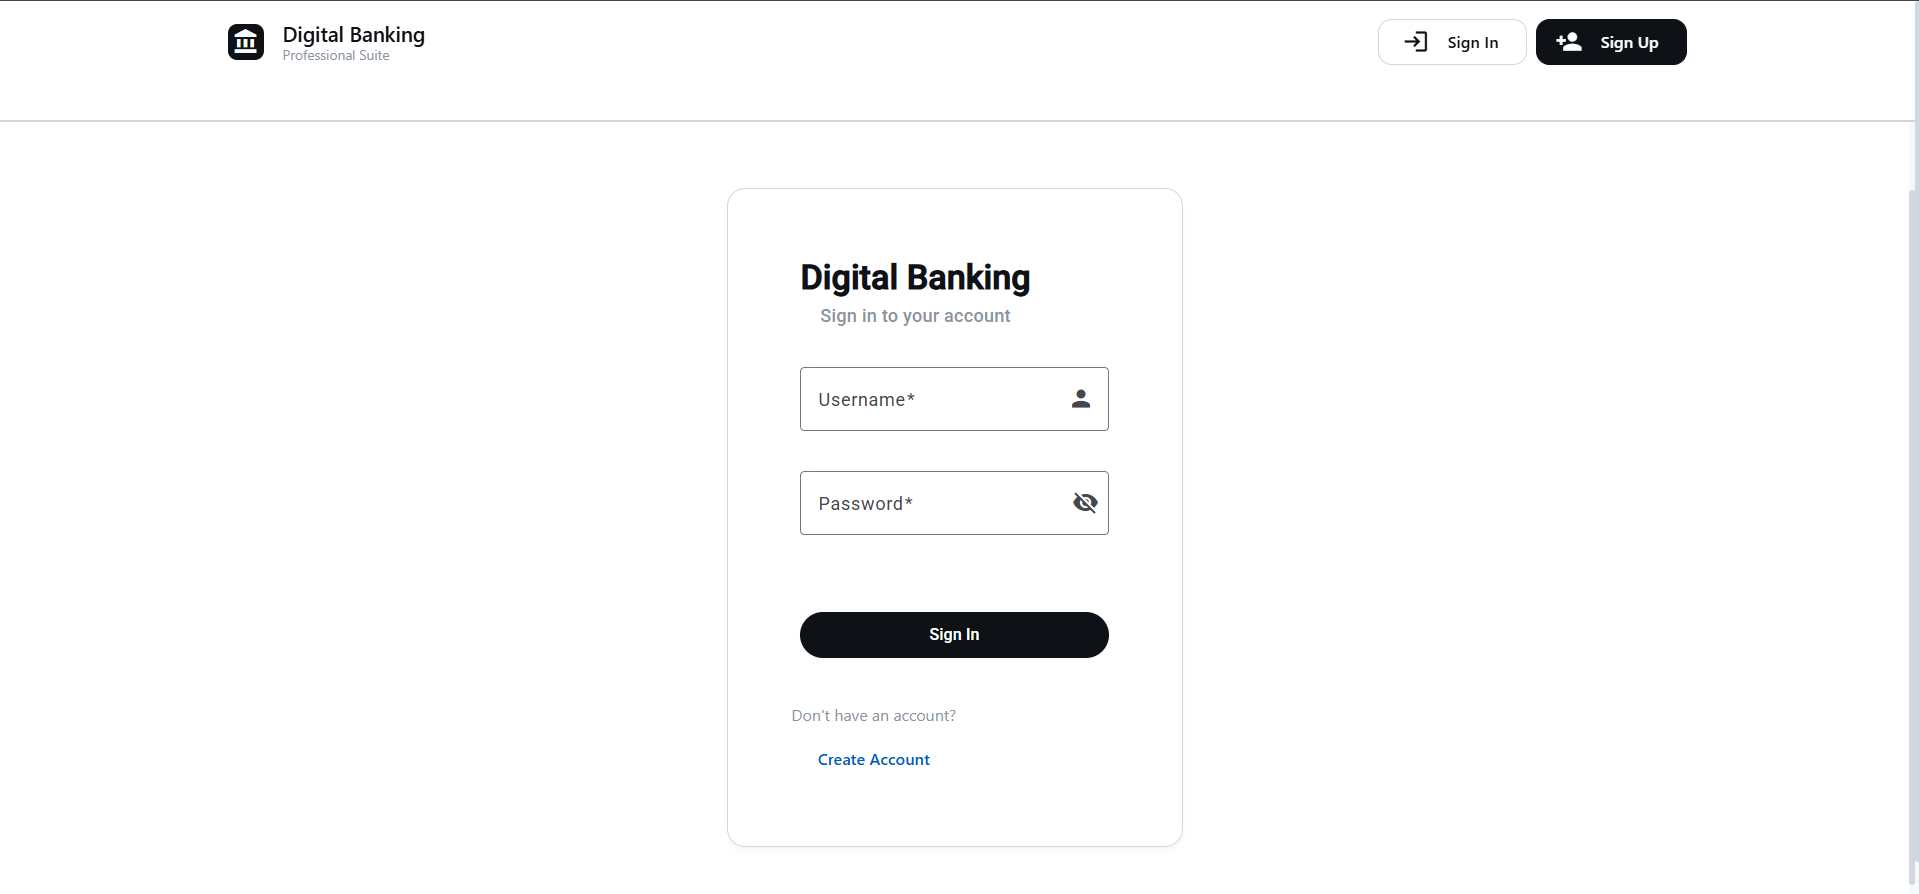
\includegraphics[width=0.8\textwidth]{screenshots/01_01_login_page_initial.png}
    \caption{\textbf{Interface de connexion initiale} - Design moderne avec champs de saisie sécurisés}
    \label{fig:login_initial}
\end{figure}

\subsection{Gestion des Erreurs d'Authentification}

Le système intègre une gestion d'erreurs claire et informative. Lorsque des identifiants incorrects sont saisis, un message d'erreur explicite guide l'utilisateur sans compromettre la sécurité.

\begin{figure}[H]
    \centering
    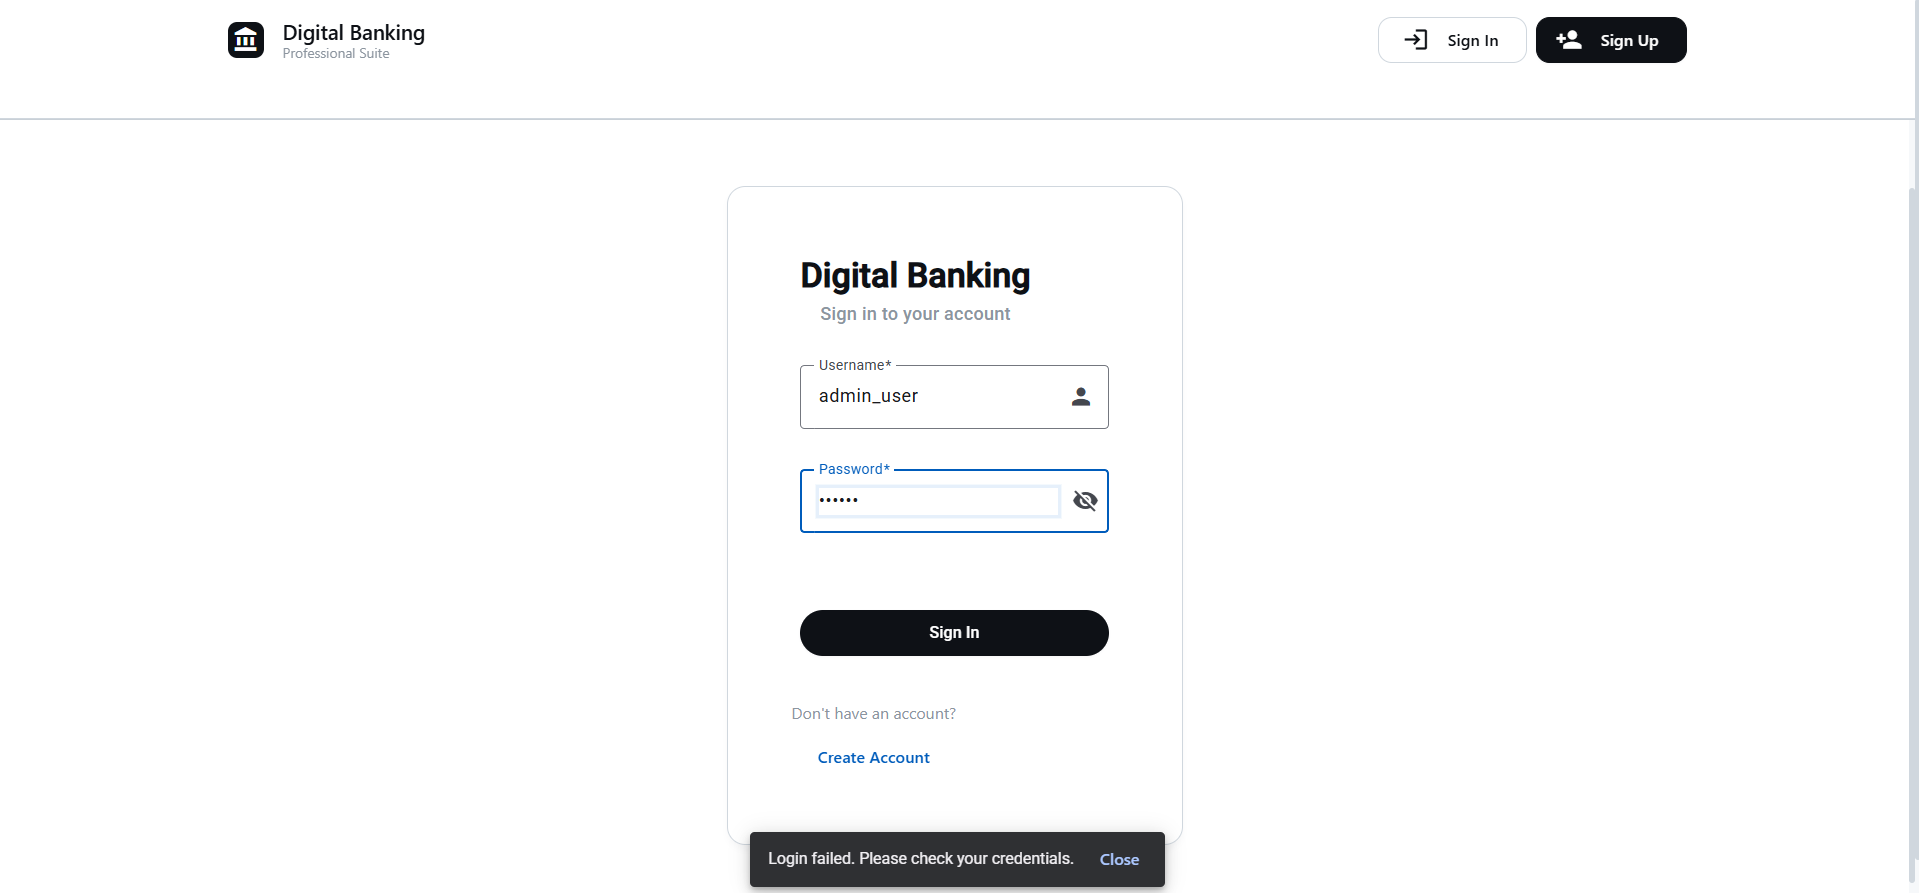
\includegraphics[width=0.8\textwidth]{screenshots/01_02_login_page_incorrect_credentials.png}
    \caption{\textbf{Gestion des erreurs} - Message d'erreur informatif en cas d'identifiants incorrects}
    \label{fig:login_incorrect}
\end{figure}

\subsection{Accès Réussi au Tableau de Bord}

Après une authentification réussie avec les identifiants valides (\texttt{admin\_user} / \texttt{123456}), l'utilisateur est automatiquement redirigé vers le tableau de bord principal, offrant une vue d'ensemble immédiate de son espace bancaire.

\begin{figure}[H]
    \centering
    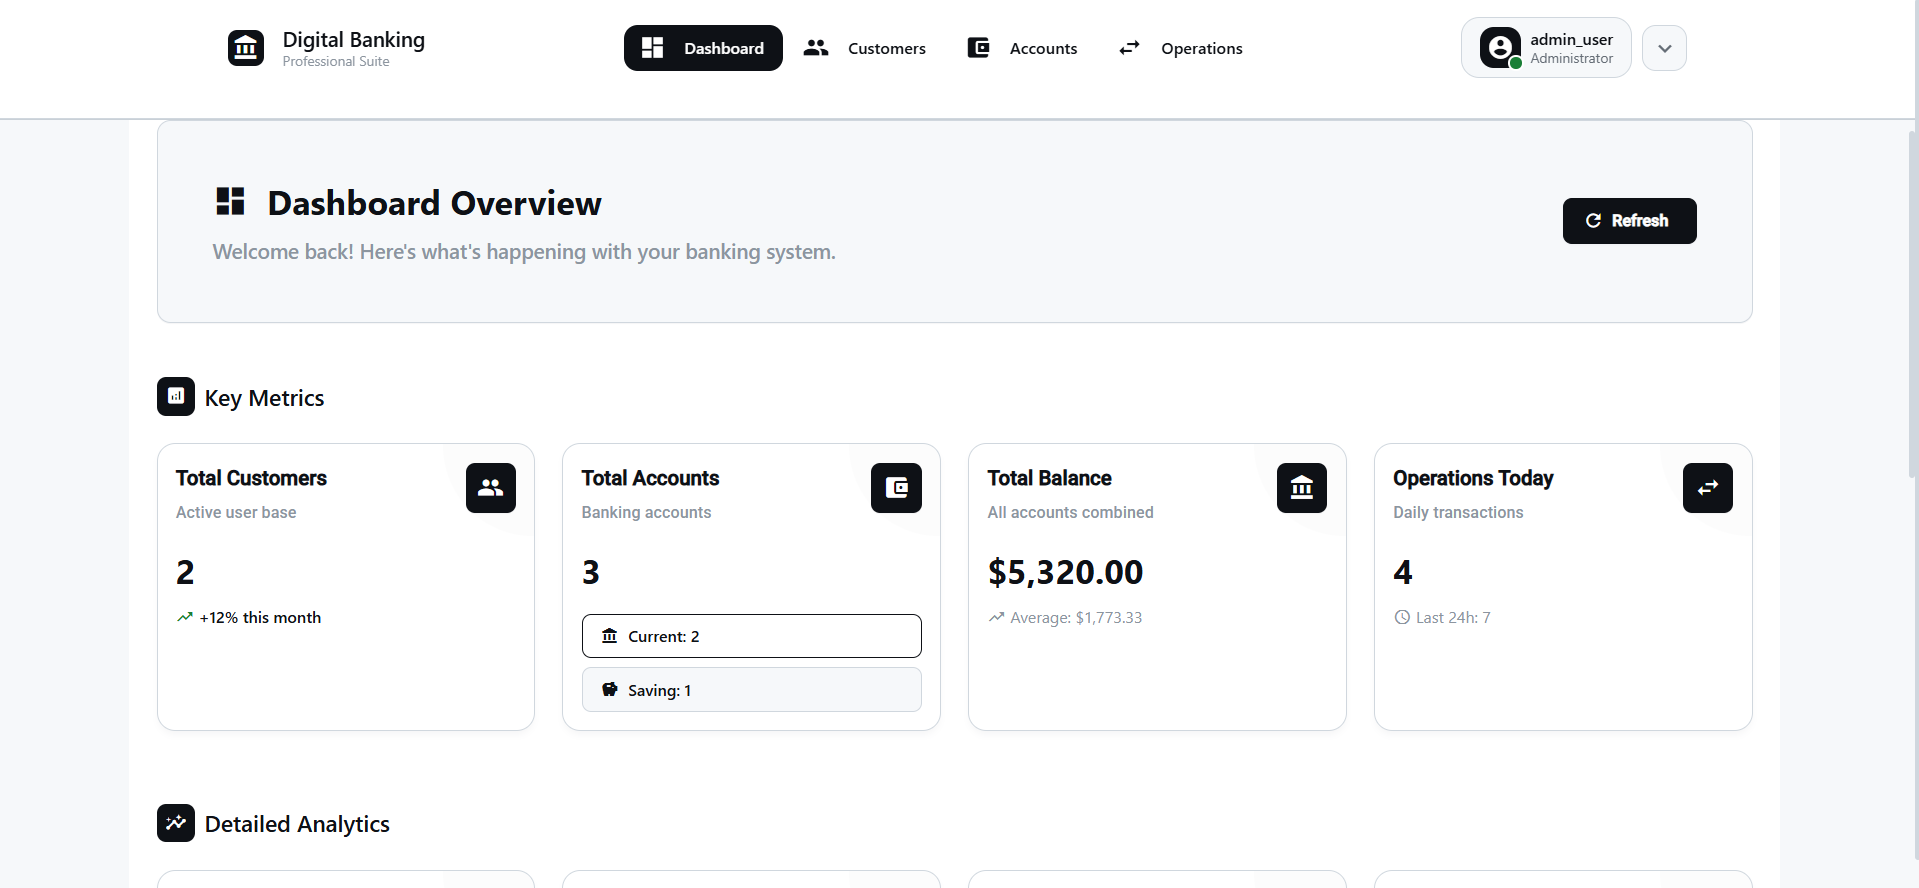
\includegraphics[width=0.8\textwidth]{screenshots/01_03_login_successful_dashboard.png}
    \caption{\textbf{Redirection post-authentification} - Accès direct au tableau de bord personnalisé}
    \label{fig:login_successful}
\end{figure}

\section{Tableau de Bord}
\accentline

\textbf{Centralisation des Informations :} Le tableau de bord constitue le centre névralgique de l'application, offrant une vue synthétique et interactive des données financières de l'utilisateur.

\subsection{Vue d'Ensemble Interactive}

Le tableau de bord présente une interface riche en informations, incluant des graphiques dynamiques qui permettent de visualiser :

\begin{itemize}[leftmargin=20pt, itemsep=3pt]
    \item \textbf{Distribution des types de comptes} : Répartition visuelle entre comptes courants et comptes d'épargne
    \item \textbf{Tendances des opérations} : Évolution temporelle des transactions
    \item \textbf{Indicateurs clés} : Métriques importantes en temps réel
    \item \textbf{Navigation rapide} : Accès direct aux fonctionnalités principales
\end{itemize}

\begin{figure}[H]
    \centering
    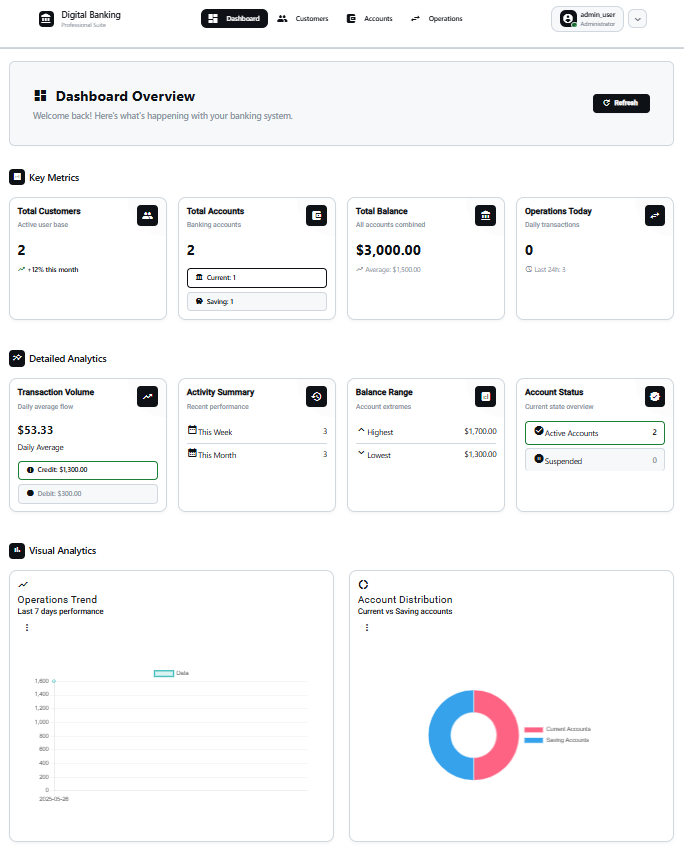
\includegraphics[width=0.9\textwidth]{screenshots/02_01_dashboard_overview.png}
    \caption{\textbf{Tableau de bord complet} - Interface centralisée avec graphiques interactifs et navigation intuitive}
    \label{fig:dashboard_overview}
\end{figure}

\section{Gestion des Clients}
\accentline

\textbf{Gestion Complète :} Module dédié à l'administration des profils clients avec fonctionnalités CRUD (Créer, Lire, Mettre à jour, Supprimer) complètes et interface intuitive.

\subsection{Consultation de la Base Clients}

L'interface de gestion présente une vue tabulaire organisée de tous les clients enregistrés dans le système, avec des options de recherche et de filtrage avancées.

\begin{figure}[H]
    \centering
    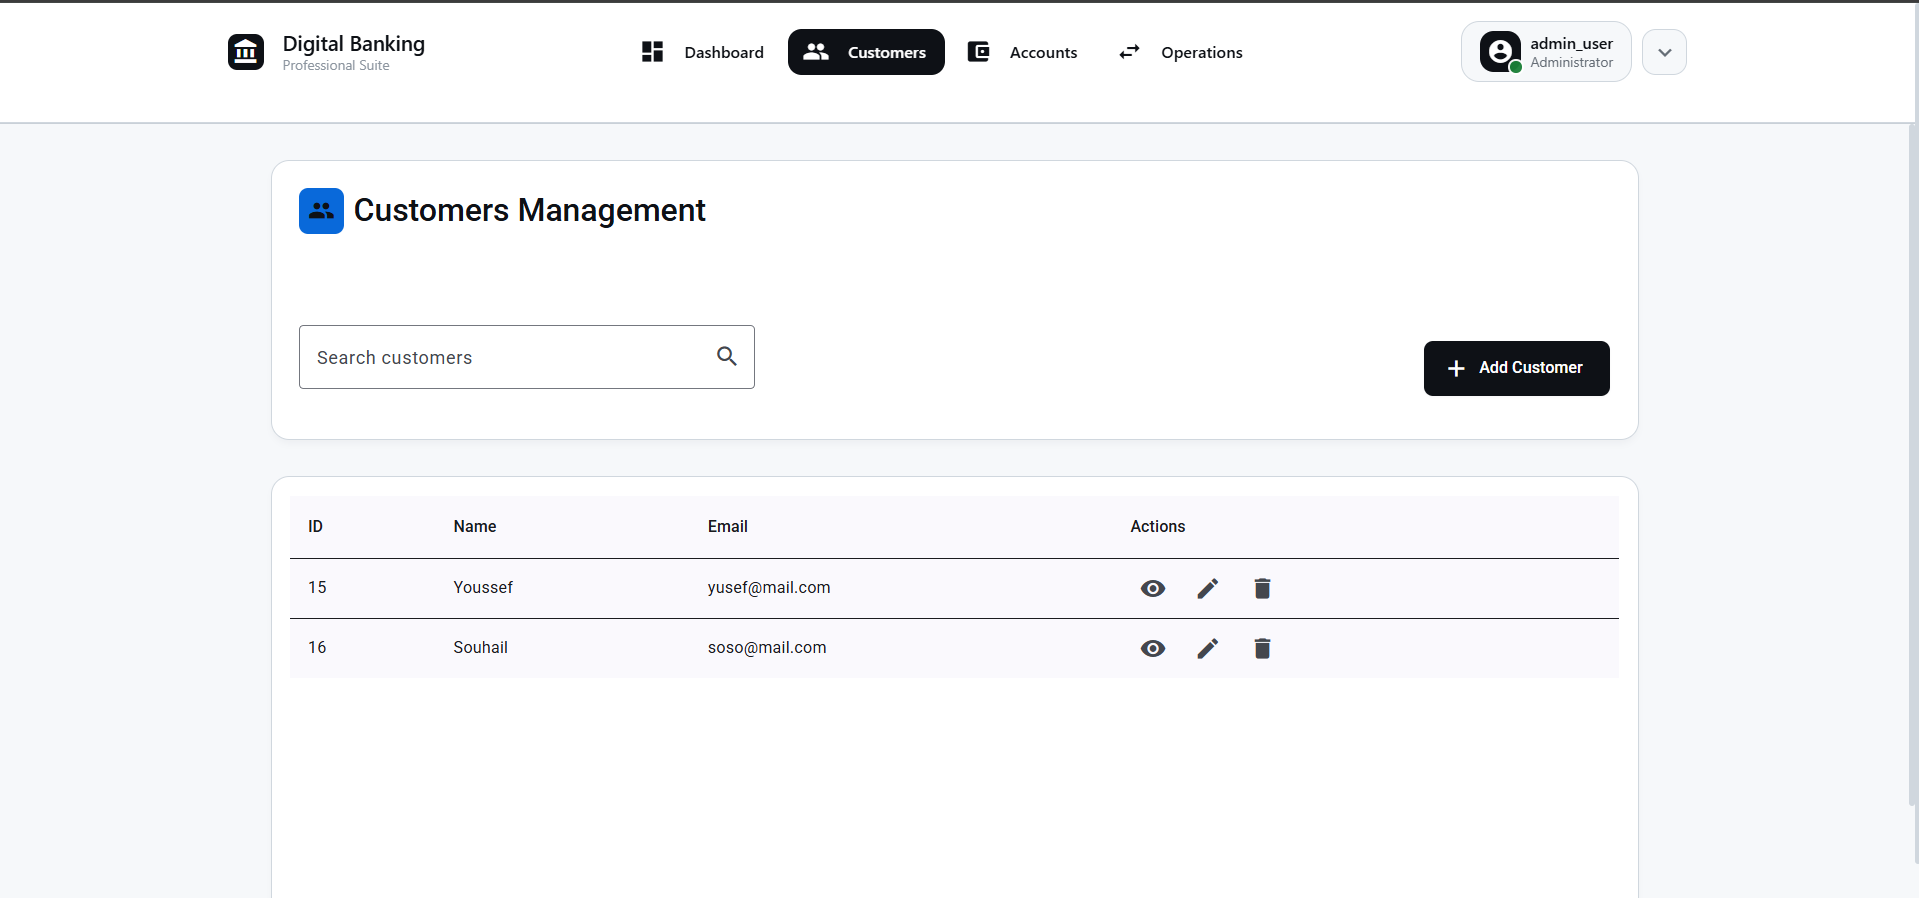
\includegraphics[width=0.9\textwidth]{screenshots/04_01_customer_list_initial.png}
    \caption{\textbf{Liste des clients} - Interface tabulaire avec fonctionnalités de recherche et actions rapides}
    \label{fig:customer_list_initial}
\end{figure}

\subsection{Création de Nouveaux Profils}

\subsubsection{Formulaire de Saisie Vierge}

L'interface de création propose un formulaire structuré et ergonomique pour la saisie des informations client.

\begin{figure}[H]
    \centering
    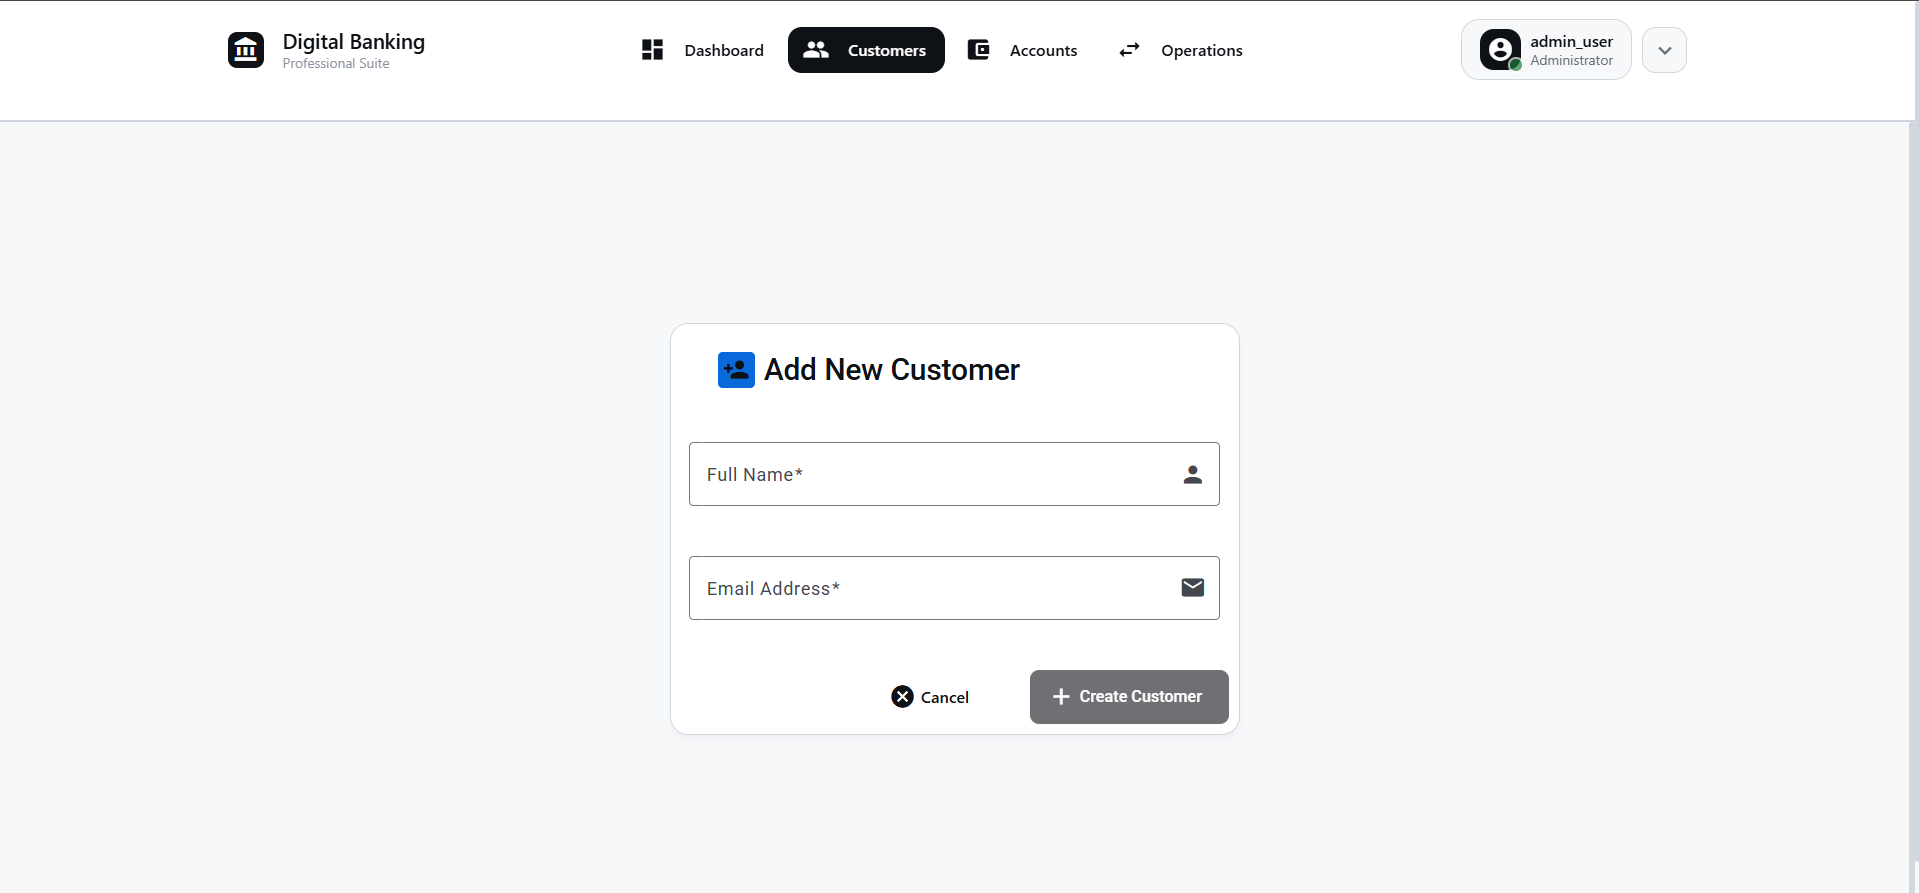
\includegraphics[width=0.75\textwidth]{screenshots/04_02_customer_form_new_empty.png}
    \caption{\textbf{Formulaire de création} - Interface de saisie vierge avec validation en temps réel}
    \label{fig:customer_form_new_empty}
\end{figure}

\subsubsection{Processus de Saisie}

Exemple de saisie avec validation des données en temps réel et assistance contextuelle.

\begin{figure}[H]
    \centering
    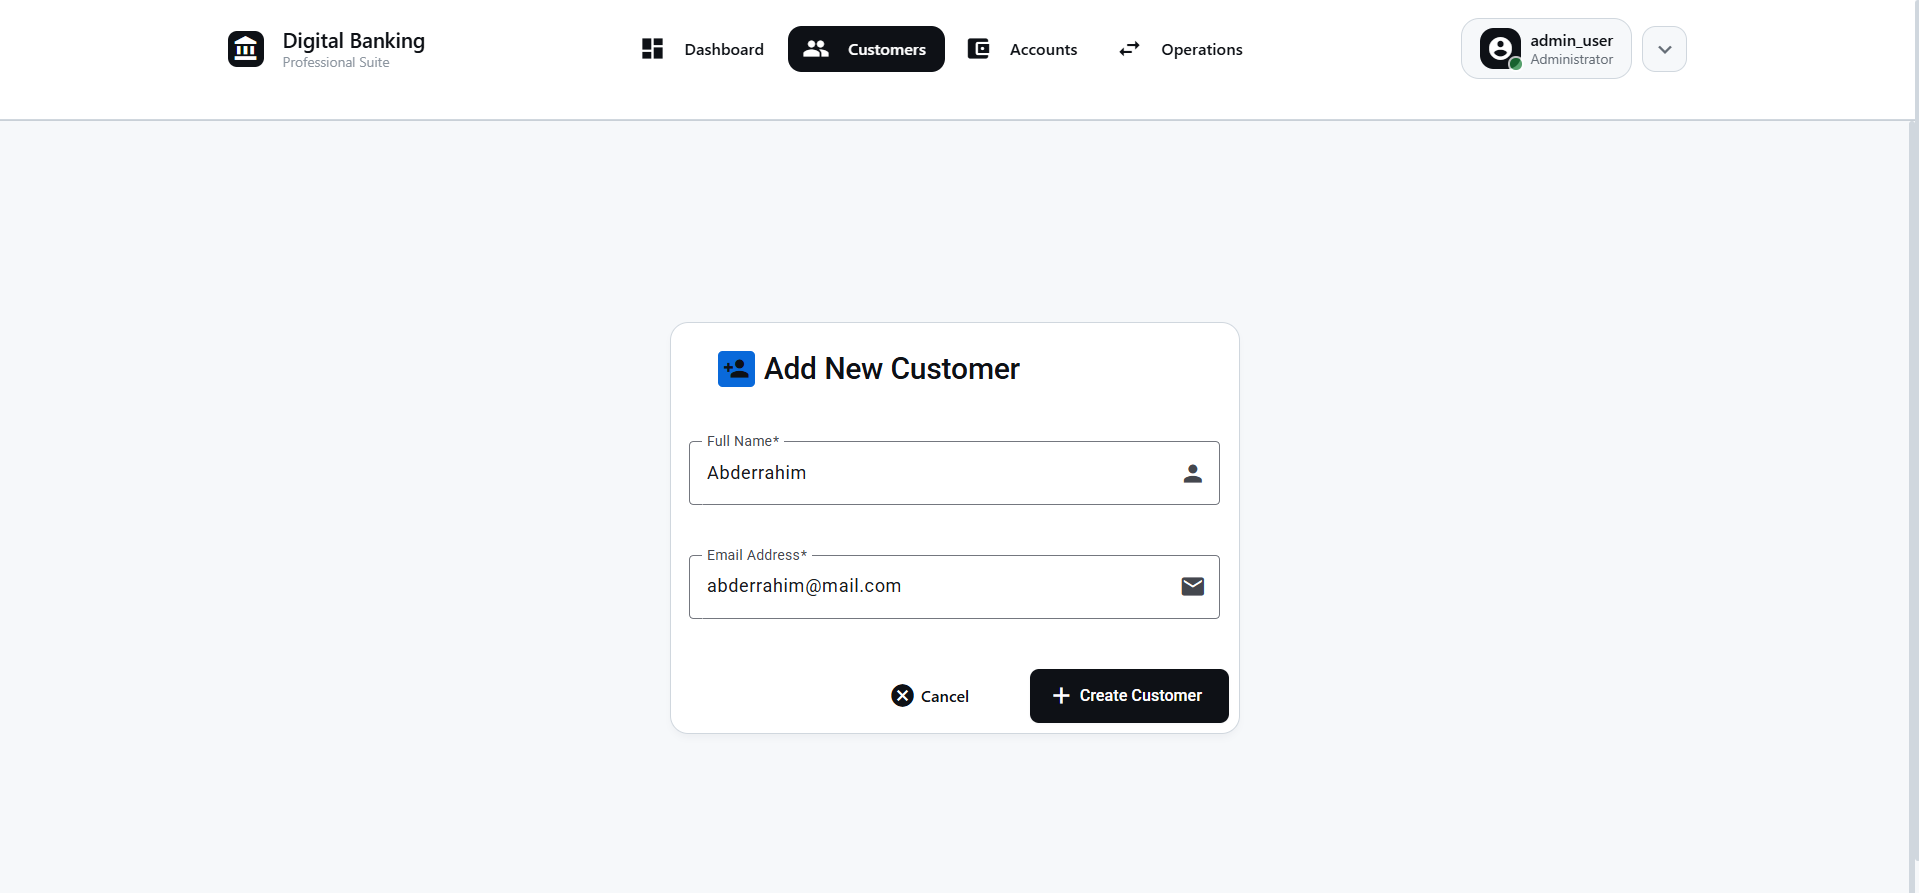
\includegraphics[width=0.75\textwidth]{screenshots/04_03_customer_form_new_filled.png}
    \caption{\textbf{Formulaire complété} - Saisie d'exemple avec validation automatique des champs}
    \label{fig:customer_form_new_filled}
\end{figure}

\subsubsection{Confirmation de Création}

Après validation du formulaire, le nouveau client apparaît dans la liste mise à jour, confirmant la réussite de l'opération.

\begin{figure}[H]
    \centering
    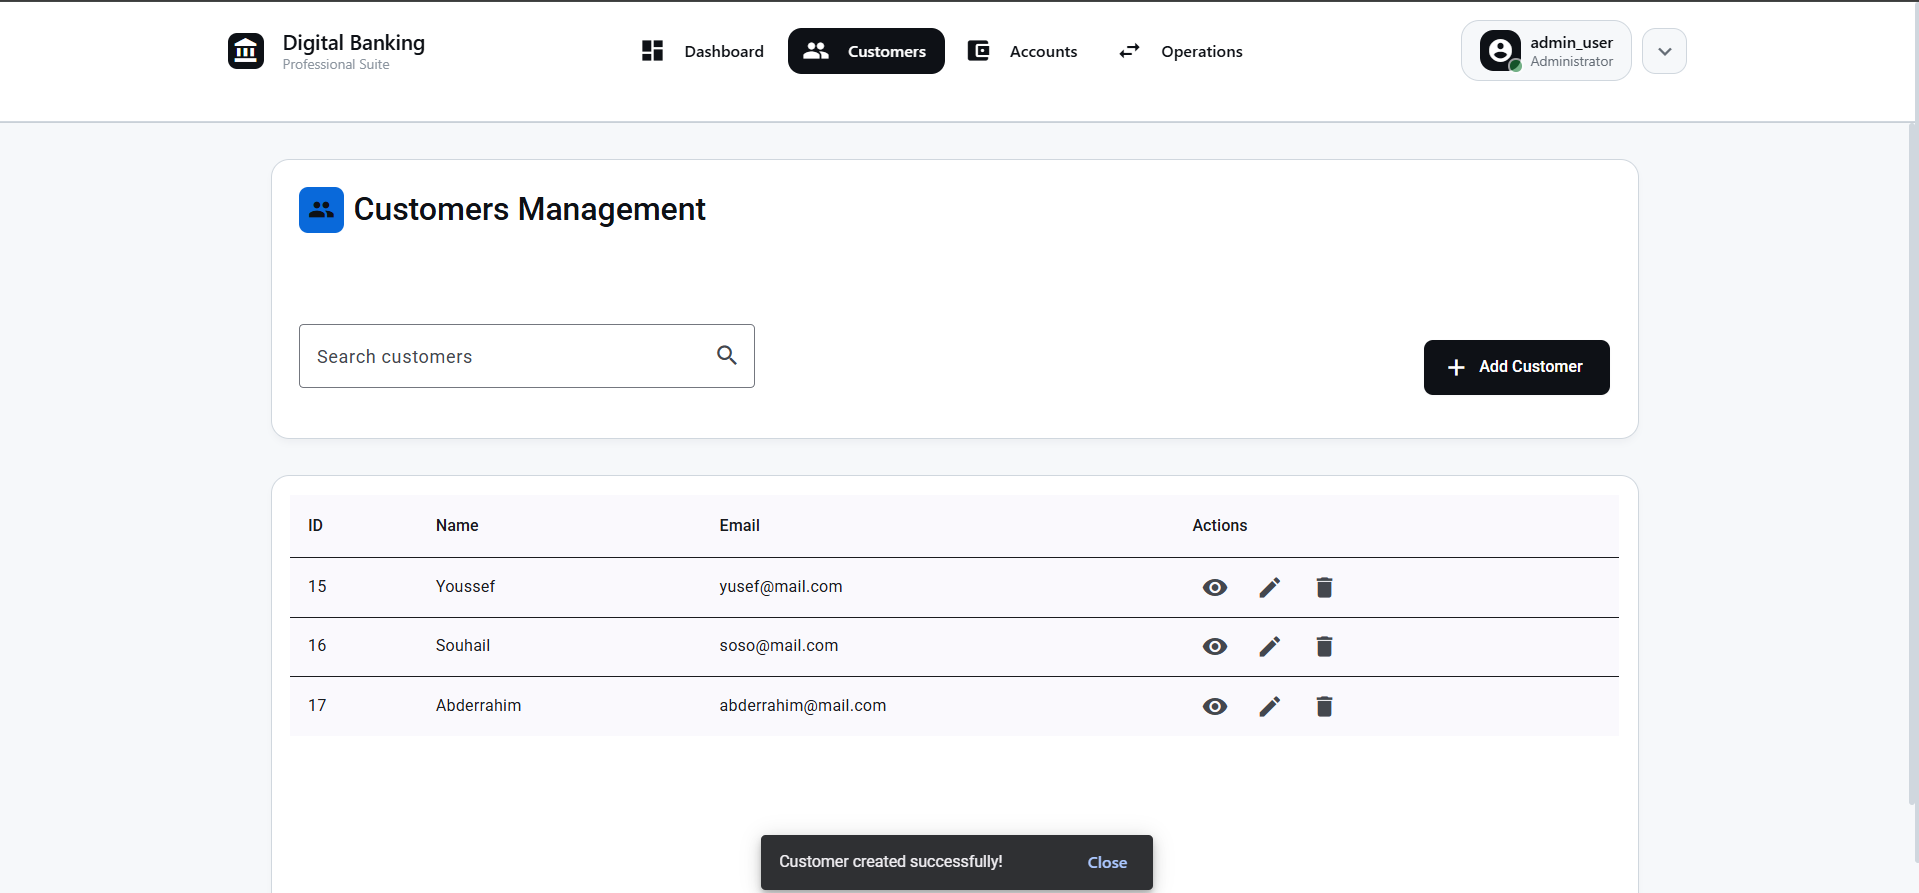
\includegraphics[width=0.9\textwidth]{screenshots/04_04_customer_list_after_creation.png}
    \caption{\textbf{Liste mise à jour} - Nouveau client ajouté avec succès à la base de données}
    \label{fig:customer_list_after_creation}
\end{figure}

\subsection{Modification des Profils Existants}

\subsubsection{Formulaire de Modification Pré-rempli}

Le système permet la modification des données clients existantes avec un formulaire pré-rempli facilitant les corrections.

\begin{figure}[H]
    \centering
    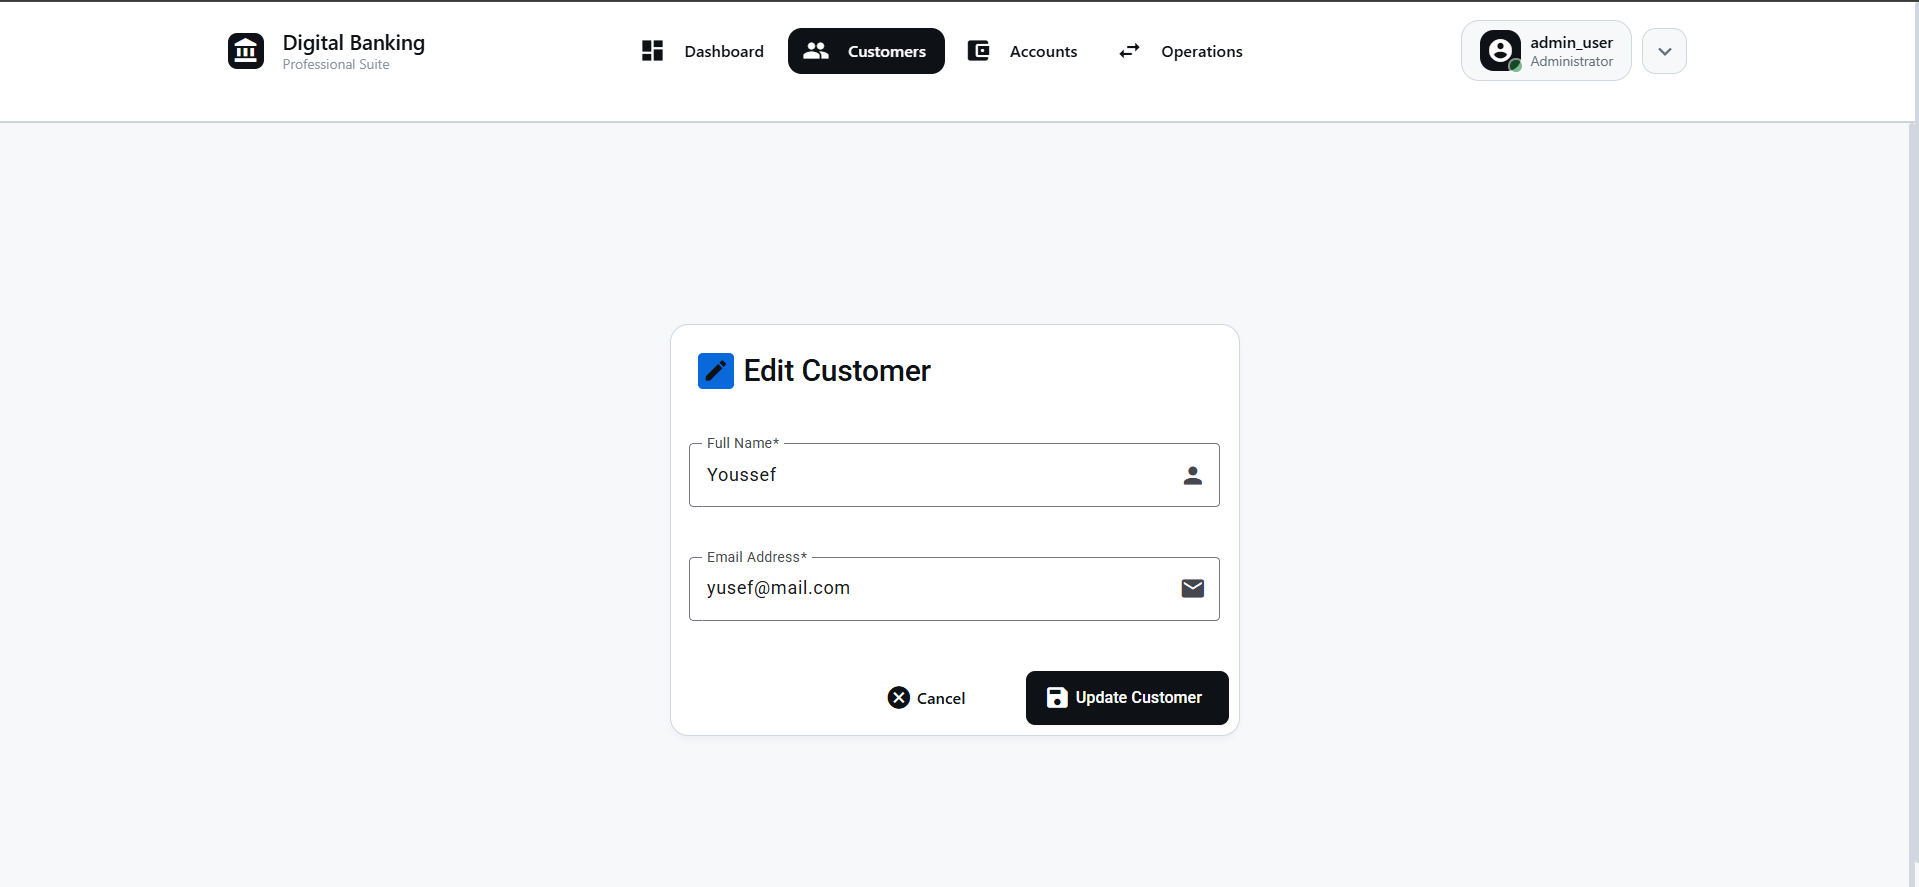
\includegraphics[width=0.75\textwidth]{screenshots/04_05_customer_form_edit_prefilled.png}
    \caption{\textbf{Formulaire de modification} - Données existantes pré-remplies pour faciliter l'édition}
    \label{fig:customer_form_edit_prefilled}
\end{figure}

\subsubsection{Mise à Jour des Informations}

Illustration du processus de modification avec les nouvelles données saisies et validation en cours.

\begin{figure}[H]
    \centering
    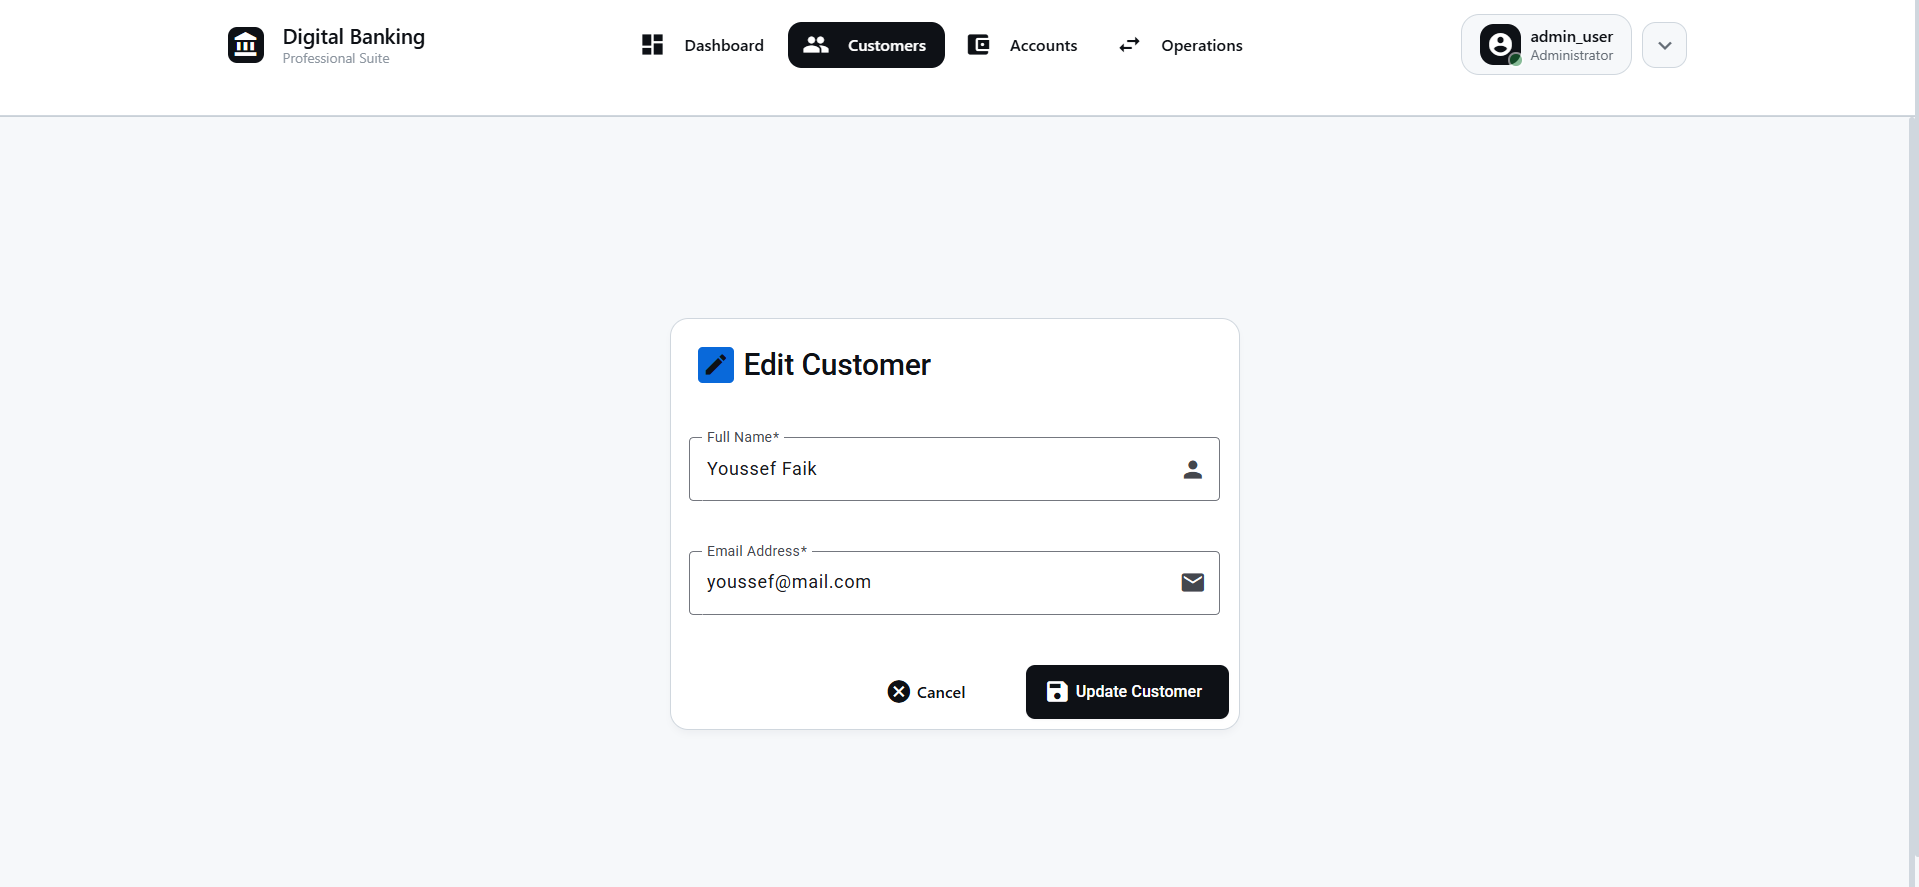
\includegraphics[width=0.75\textwidth]{screenshots/04_06_customer_form_edit_filled.png}
    \caption{\textbf{Formulaire modifié} - Nouvelles données saisies avec validation active}
    \label{fig:customer_form_edit_filled}
\end{figure}

\subsubsection{Confirmation de Mise à Jour}

La liste des clients reflète immédiatement les modifications apportées, confirmant la mise à jour réussie.

\begin{figure}[H]
    \centering
    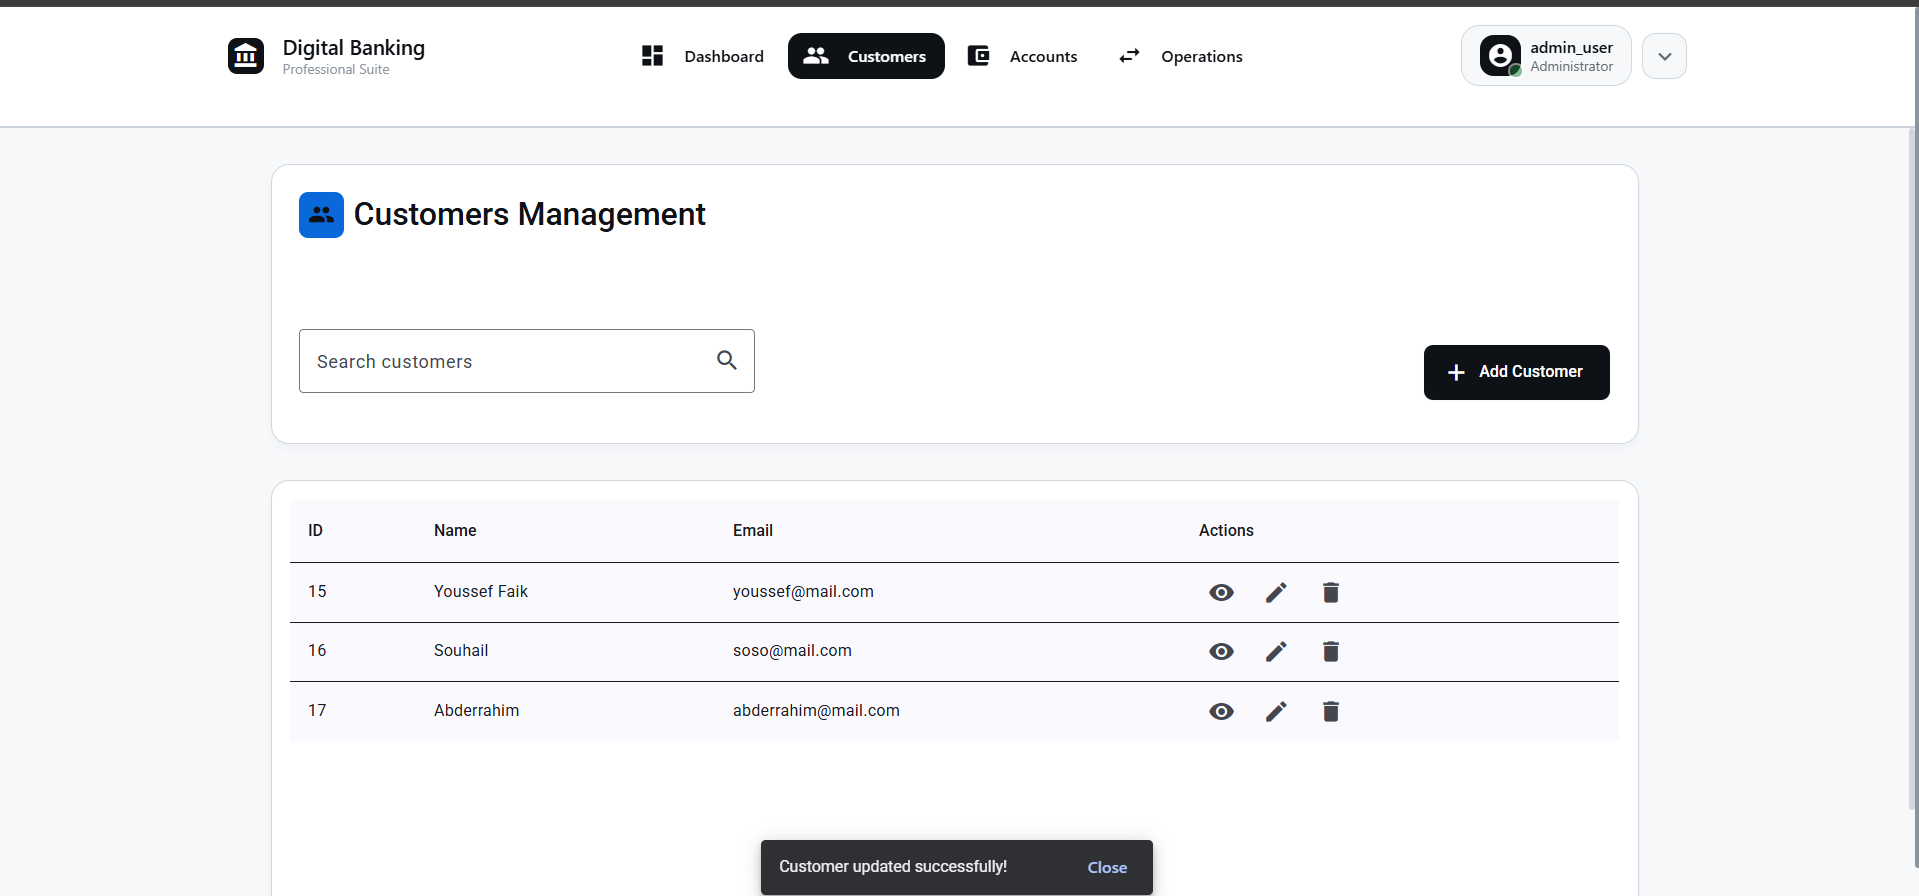
\includegraphics[width=0.9\textwidth]{screenshots/04_07_customer_list_after_update.png}
    \caption{\textbf{Liste après modification} - Données client mises à jour et visible dans l'interface}
    \label{fig:customer_list_after_update}
\end{figure}

\subsection{Suppression de Profils}

Le système permet la suppression sécurisée des profils clients avec mise à jour immédiate de la liste.

\begin{figure}[H]
    \centering
    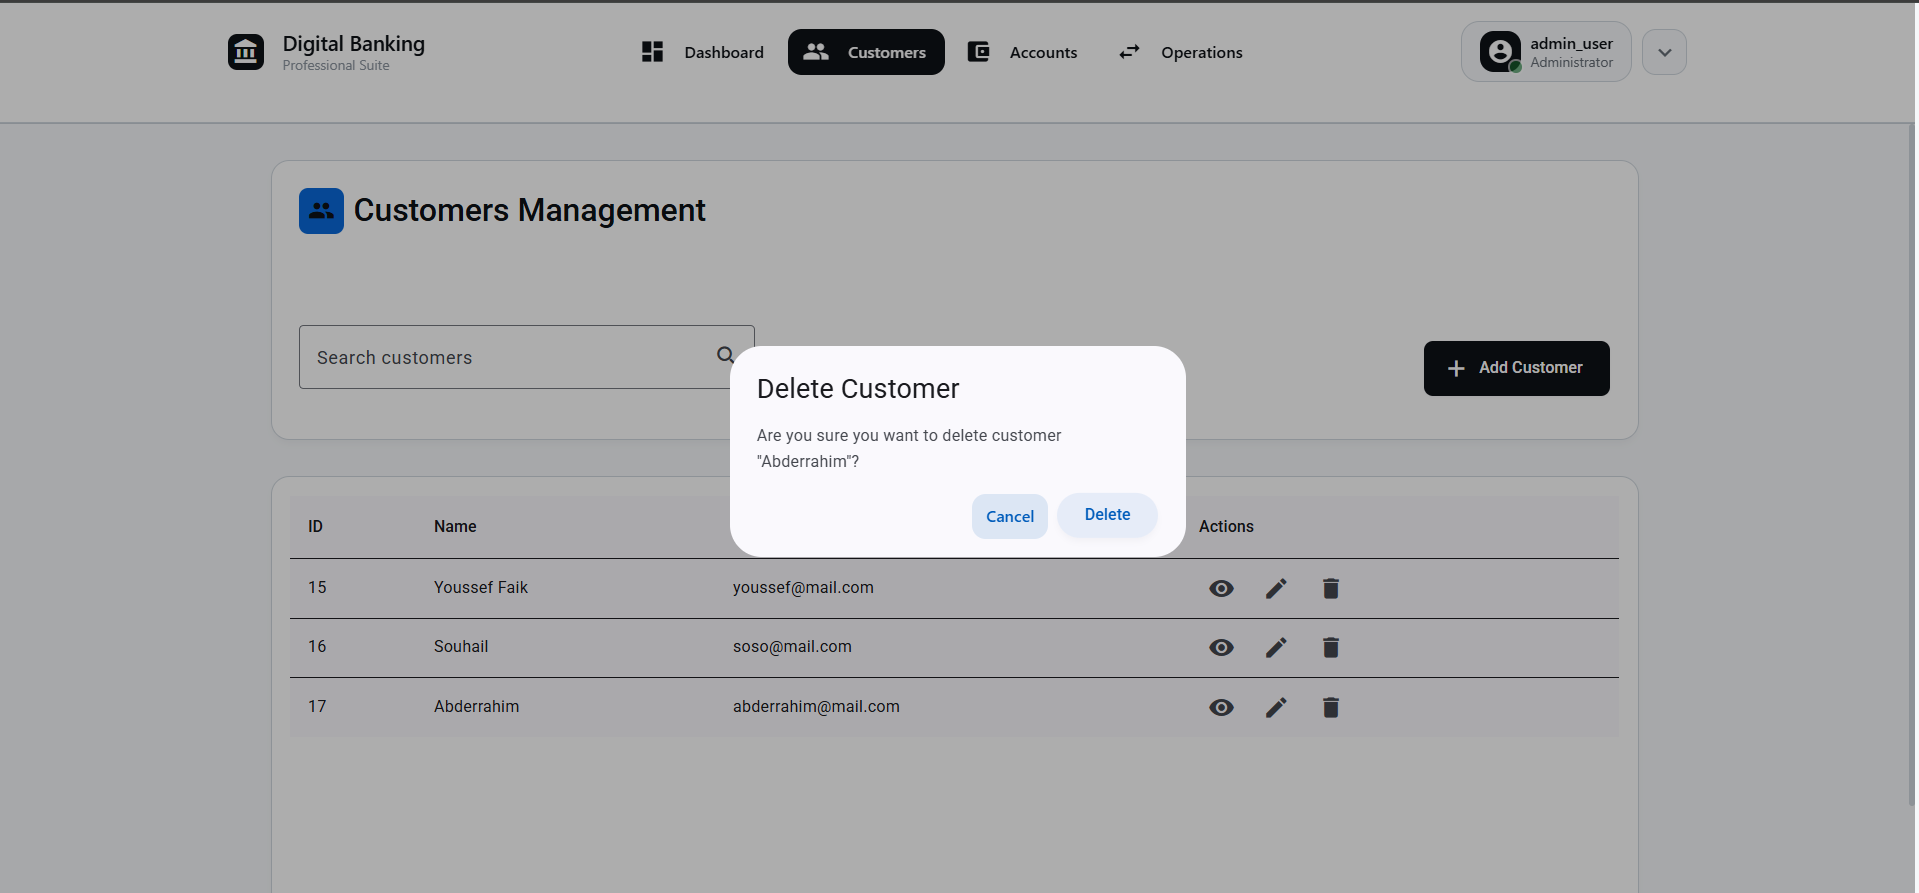
\includegraphics[width=0.9\textwidth]{screenshots/04_08_customer_list_after_delete.png}
    \caption{\textbf{Liste après suppression} - Interface mise à jour après suppression d'un profil client}
    \label{fig:customer_list_after_delete}
\end{figure}

\section{Gestion des Comptes Bancaires}
\accentline

\textbf{Administration Complète :} Module de gestion des comptes bancaires avec création, consultation et administration des comptes clients.

\subsection{Liste des Comptes Existants}

L'interface présente tous les comptes bancaires enregistrés avec leurs informations principales.

\begin{figure}[H]
    \centering
    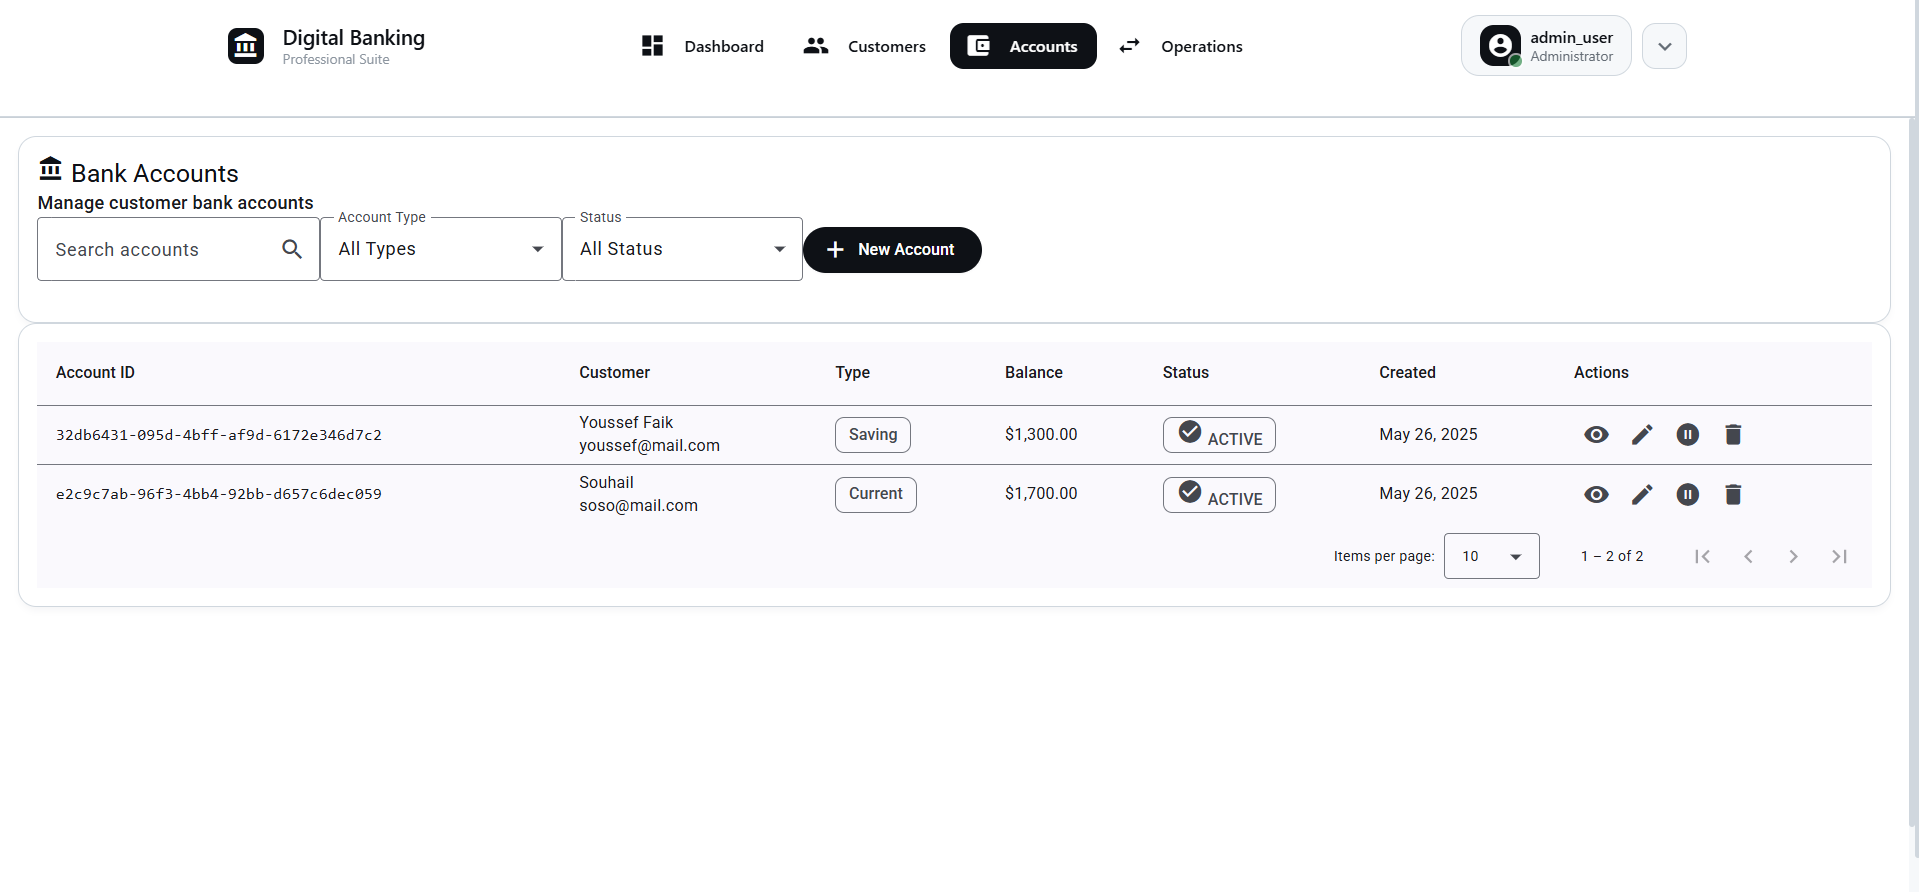
\includegraphics[width=0.9\textwidth]{screenshots/05_01_account_list_initial.png}
    \caption{\textbf{Liste des comptes} - Vue d'ensemble des comptes bancaires avec informations essentielles}
    \label{fig:account_list_initial}
\end{figure}

\subsection{Création de Nouveaux Comptes}

\subsubsection{Formulaire de Création Vierge}

Interface dédiée à la création de nouveaux comptes bancaires avec sélection du type de compte et paramètres initiaux.

\begin{figure}[H]
    \centering
    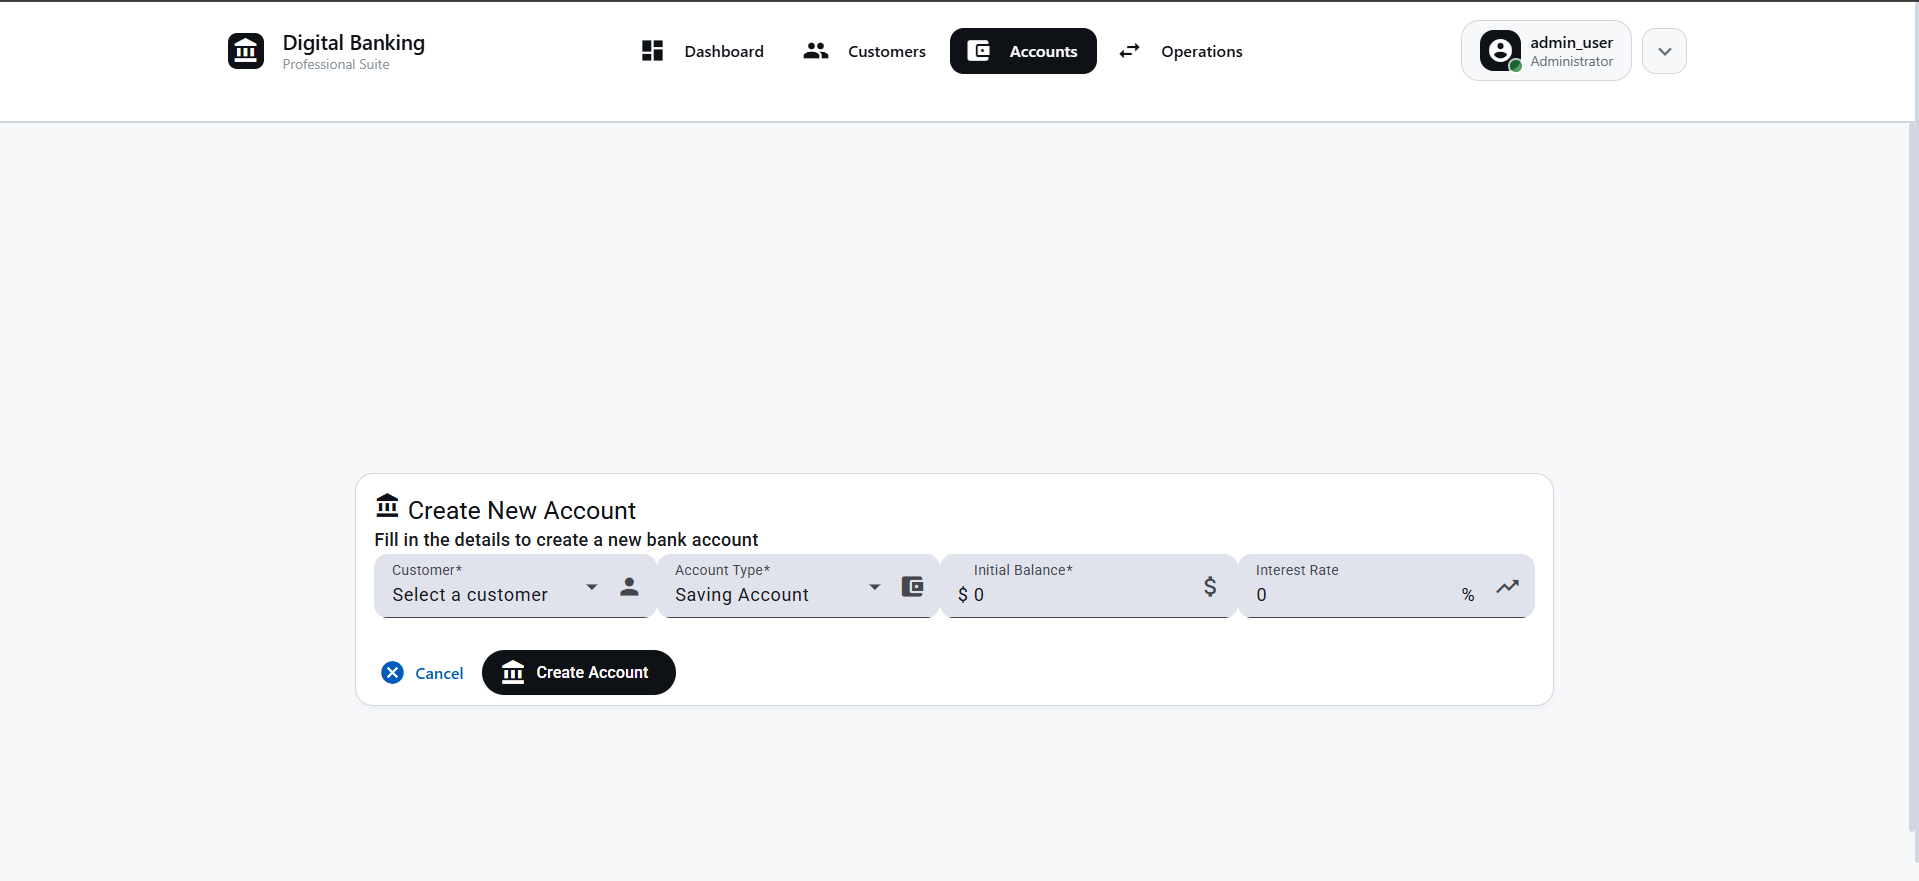
\includegraphics[width=0.75\textwidth]{screenshots/05_02_account_form_new_empty.png}
    \caption{\textbf{Formulaire de création de compte} - Interface de saisie pour nouveau compte bancaire}
    \label{fig:account_form_new_empty}
\end{figure}

\subsubsection{Paramétrage du Compte}

Exemple de création d'un compte courant avec solde initial de 1500€ et sélection du client propriétaire.

\begin{figure}[H]
    \centering
    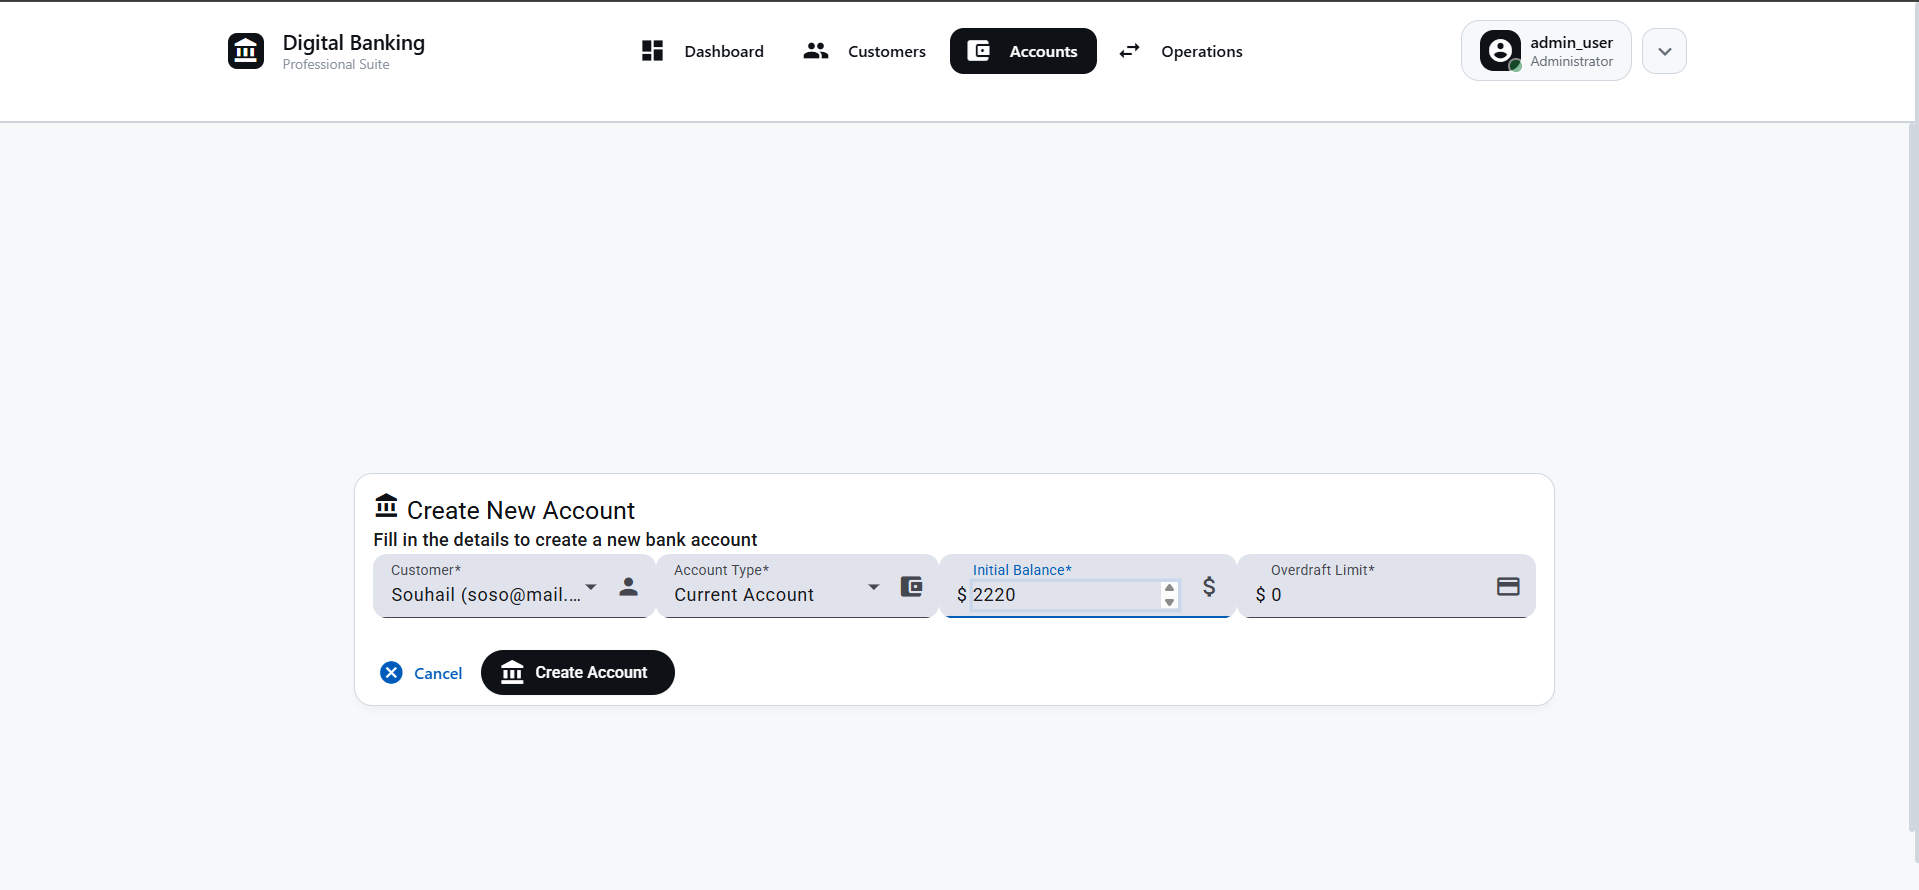
\includegraphics[width=0.75\textwidth]{screenshots/05_03_account_form_new_filled.png}
    \caption{\textbf{Formulaire complété} - Paramètres définis pour création du compte courant}
    \label{fig:account_form_new_filled}
\end{figure}

\subsubsection{Confirmation de Création}

Le nouveau compte apparaît dans la liste mise à jour avec tous ses paramètres configurés.

\begin{figure}[H]
    \centering
    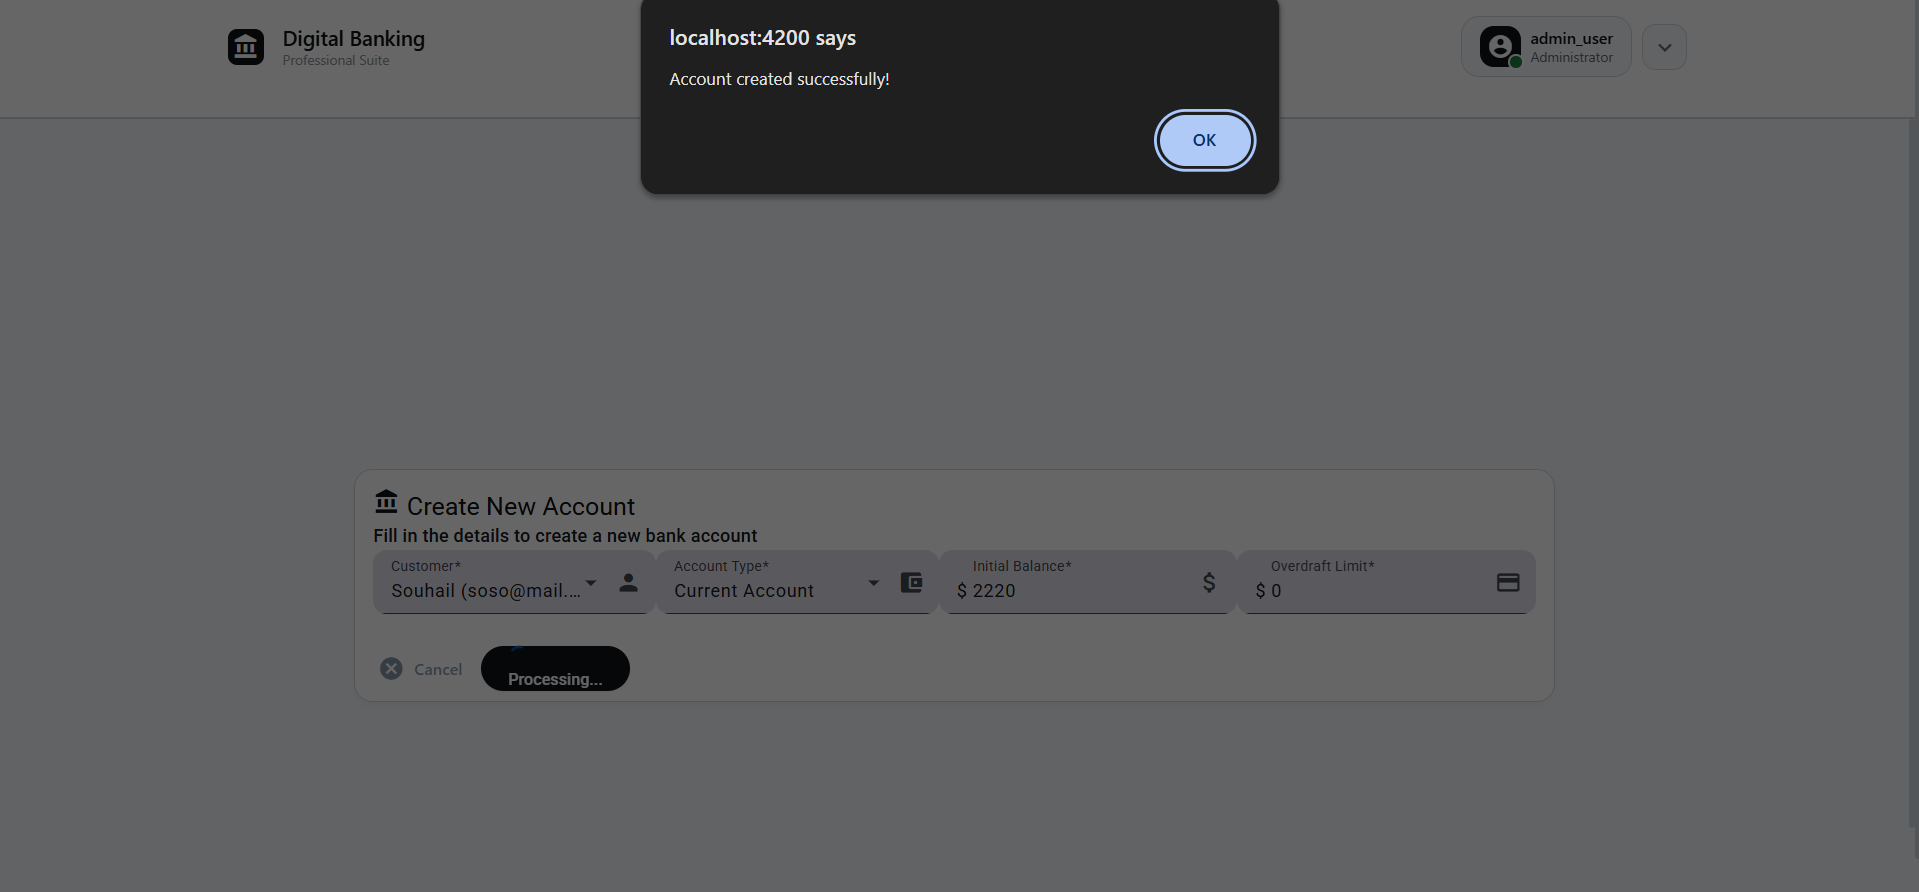
\includegraphics[width=0.9\textwidth]{screenshots/05_04_account_list_after_creation.png}
    \caption{\textbf{Liste mise à jour} - Nouveau compte créé et visible dans l'interface}
    \label{fig:account_list_after_creation}
\end{figure}

\subsection{Consultation Détaillée des Comptes}

Interface de consultation détaillée d'un compte spécifique avec historique des opérations.

\begin{figure}[H]
    \centering
    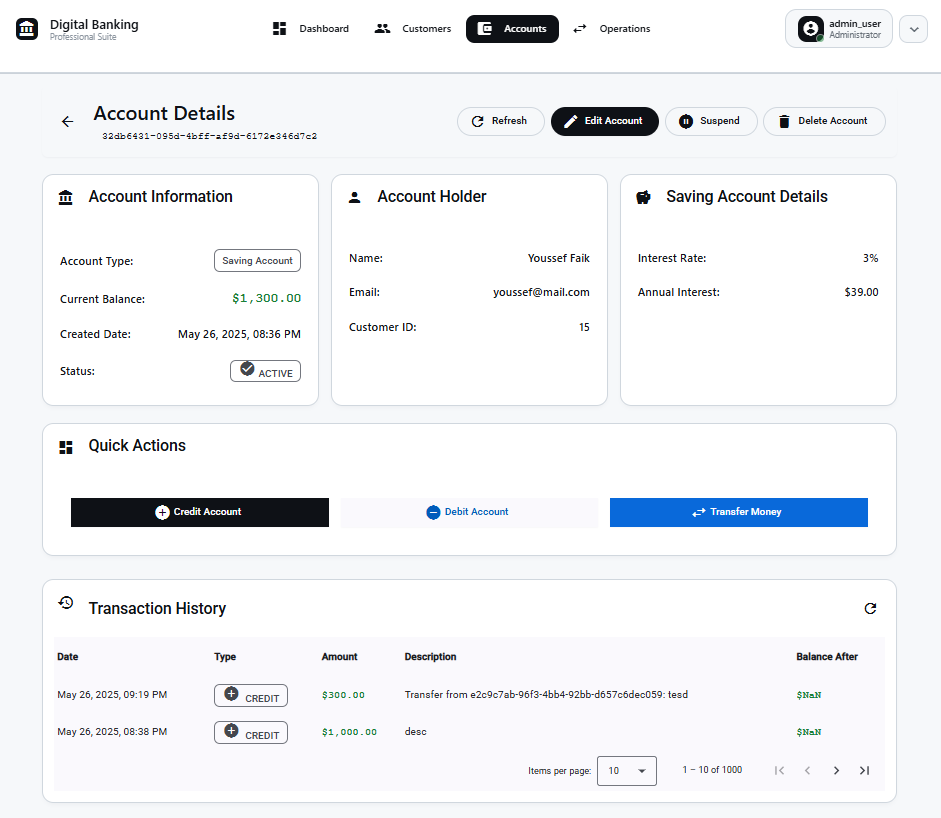
\includegraphics[width=0.9\textwidth]{screenshots/05_05_account_details_view.png}
    \caption{\textbf{Détails du compte} - Vue détaillée avec historique et informations complètes}
    \label{fig:account_details_view}
\end{figure}

\section{Opérations Bancaires}
\accentline

\textbf{Transactions Complètes :} Module de gestion des opérations bancaires incluant débit, crédit et virement avec suivi en temps réel.

\subsection{Opérations de Débit}

\subsubsection{Formulaire de Débit}

Interface pour effectuer des opérations de débit sur un compte sélectionné.

\begin{figure}[H]
    \centering
    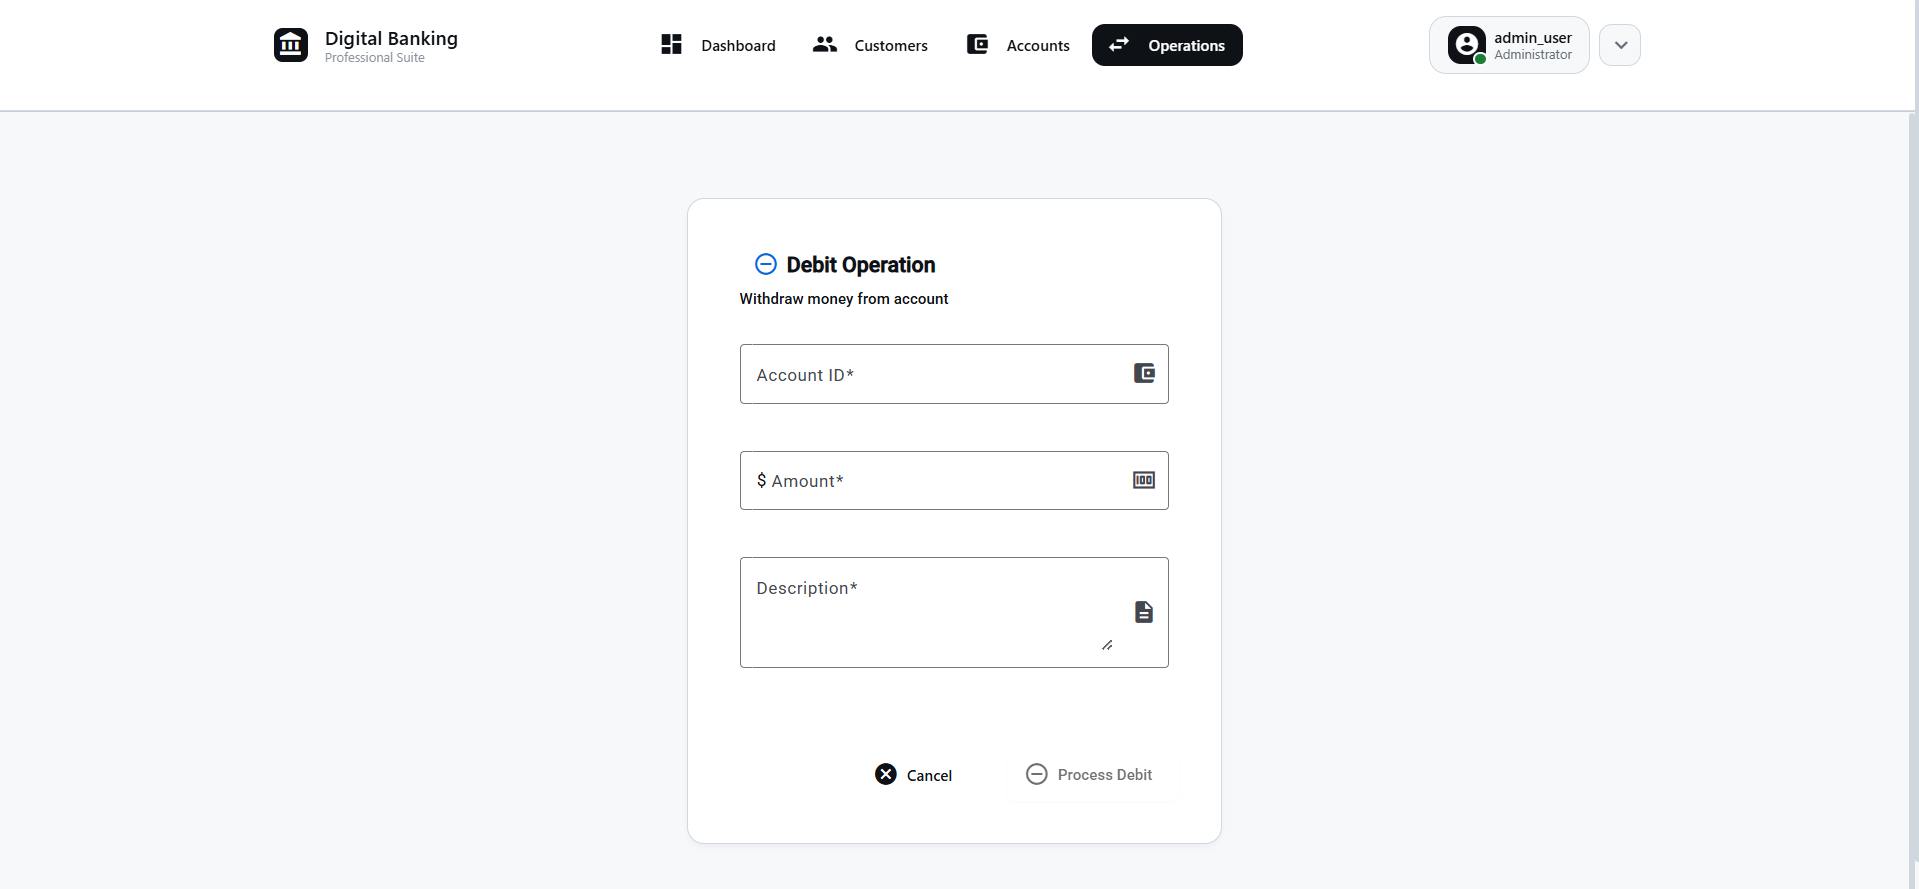
\includegraphics[width=0.75\textwidth]{screenshots/06_01_operation_debit_form_empty.png}
    \caption{\textbf{Formulaire de débit} - Interface pour saisir une opération de débit}
    \label{fig:operation_debit_form_empty}
\end{figure}

\subsubsection{Saisie de l'Opération}

Exemple de débit de 500€ avec description détaillée de l'opération.

\begin{figure}[H]
    \centering
    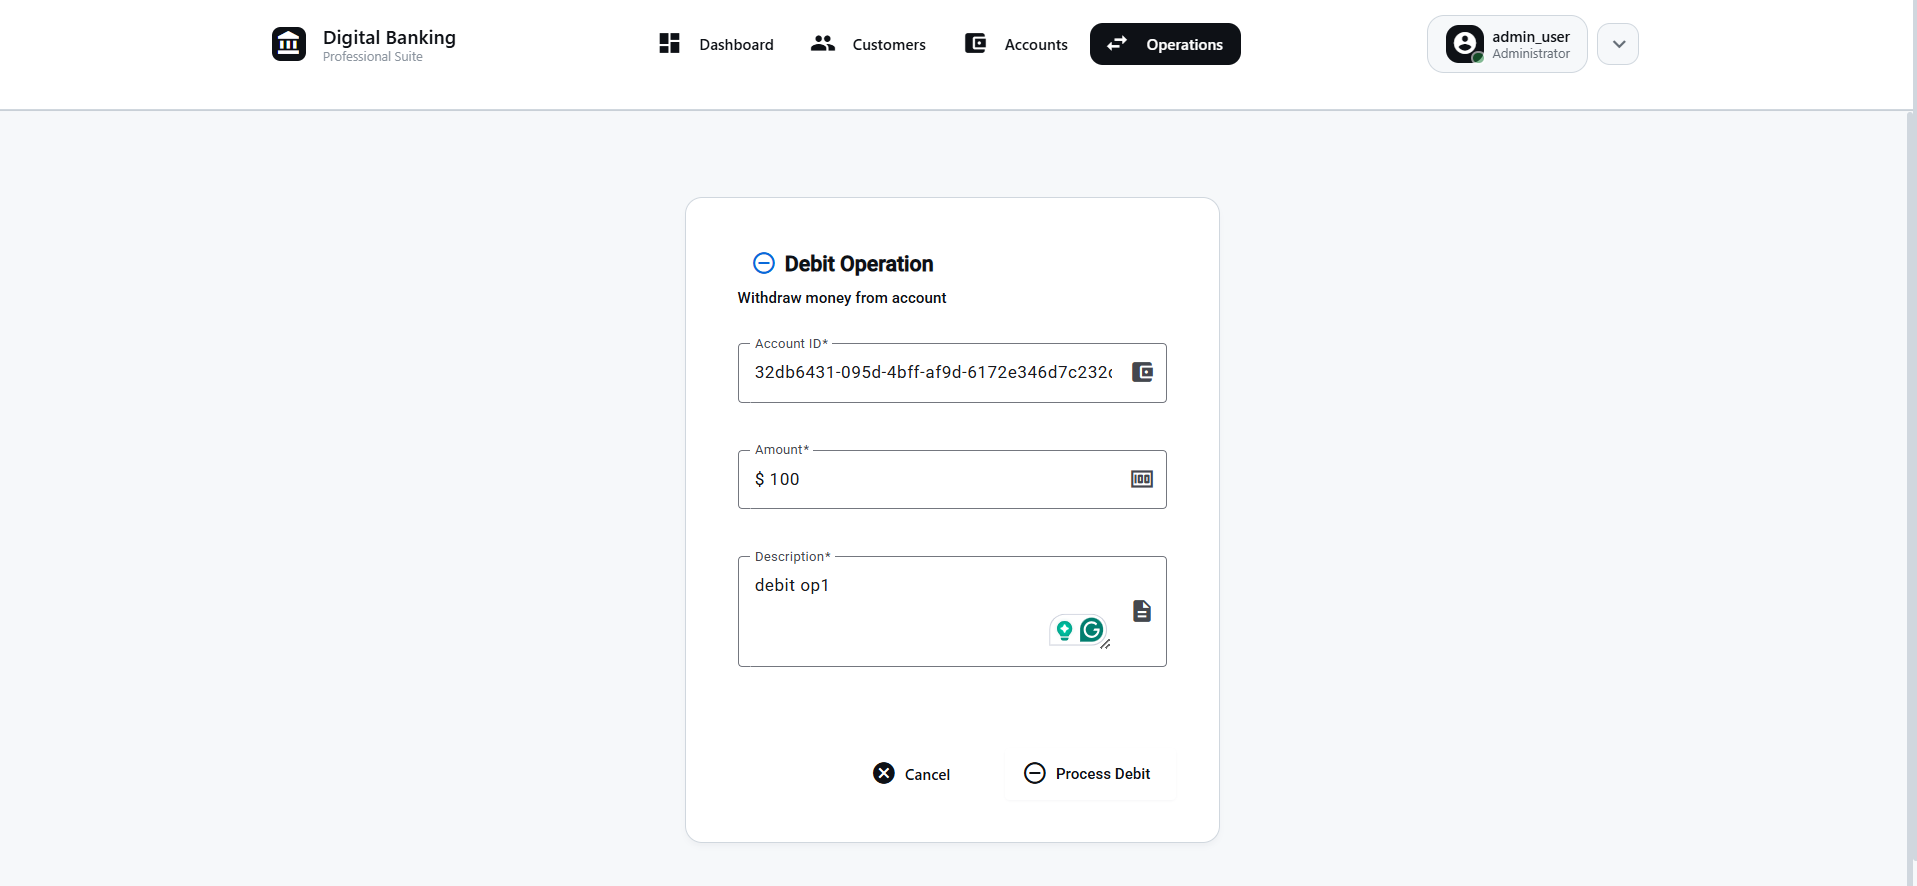
\includegraphics[width=0.75\textwidth]{screenshots/06_02_operation_debit_form_filled.png}
    \caption{\textbf{Opération de débit saisie} - Formulaire complété avec montant et description}
    \label{fig:operation_debit_form_filled}
\end{figure}

\subsubsection{État du Compte Après Débit}

Visualisation du compte après l'opération de débit avec solde mis à jour et historique enrichi.

\begin{figure}[H]
    \centering
    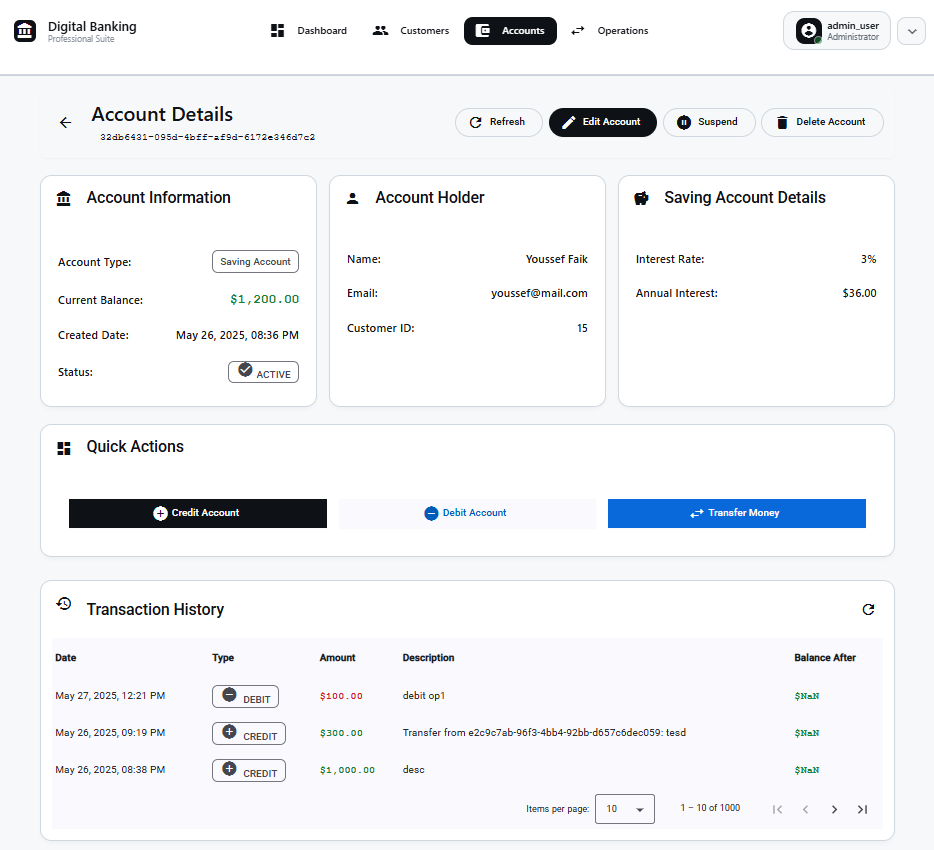
\includegraphics[width=0.9\textwidth]{screenshots/06_03_account_details_after_debit.png}
    \caption{\textbf{Compte après débit} - Solde mis à jour et opération enregistrée dans l'historique}
    \label{fig:account_details_after_debit}
\end{figure}

\subsection{Opérations de Crédit}

\subsubsection{Formulaire de Crédit}

Interface dédiée aux opérations de crédit pour alimenter un compte bancaire.

\begin{figure}[H]
    \centering
    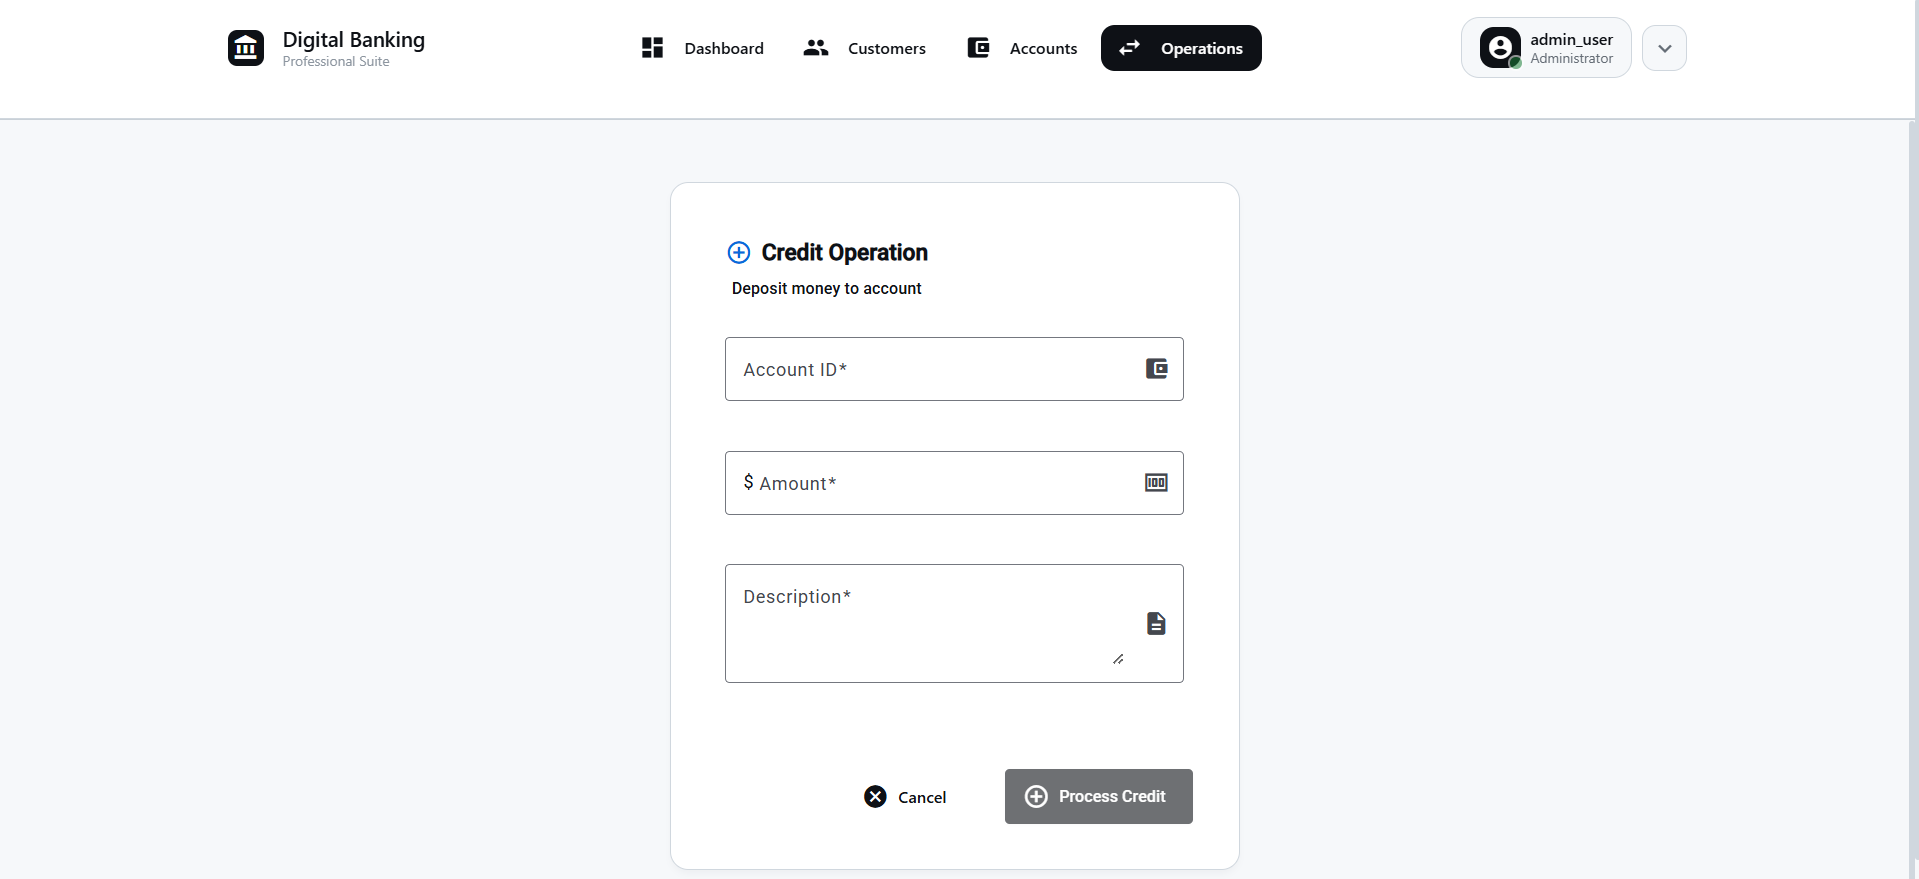
\includegraphics[width=0.75\textwidth]{screenshots/06_04_operation_credit_form_empty.png}
    \caption{\textbf{Formulaire de crédit} - Interface pour effectuer un crédit sur le compte}
    \label{fig:operation_credit_form_empty}
\end{figure}

\subsubsection{Exécution du Crédit}

Exemple de crédit de 1000€ avec description de l'origine des fonds.

\begin{figure}[H]
    \centering
    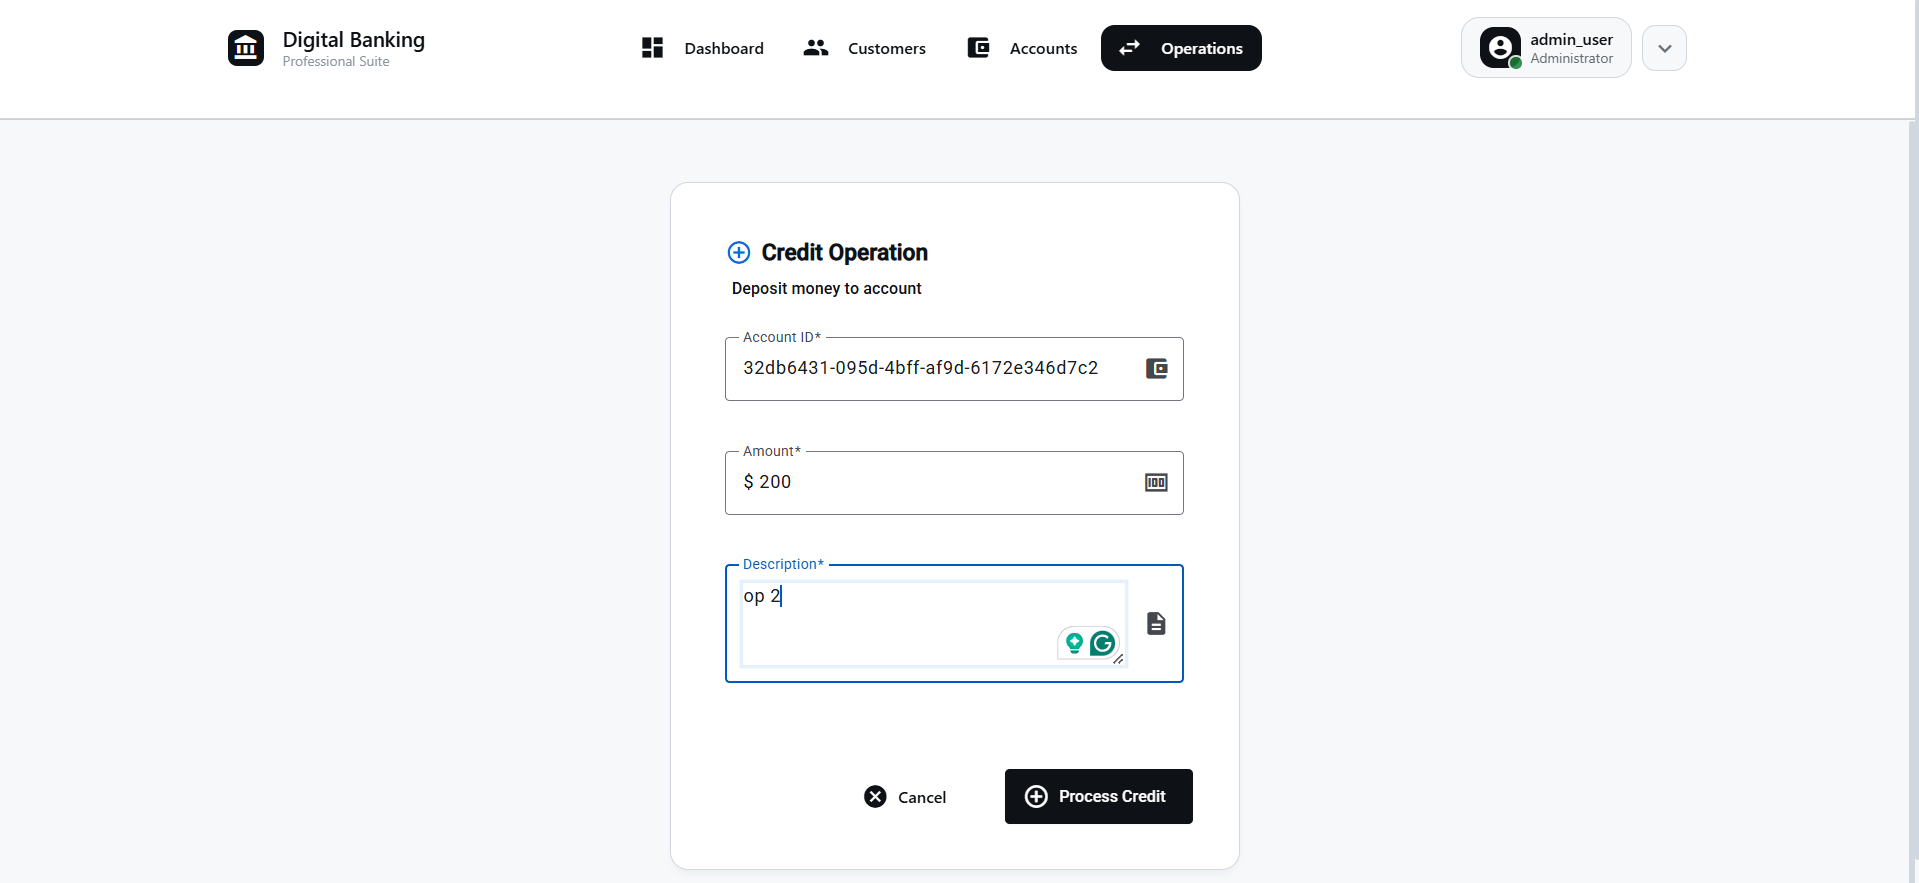
\includegraphics[width=0.75\textwidth]{screenshots/06_05_operation_credit_form_filled.png}
    \caption{\textbf{Opération de crédit} - Formulaire rempli avec montant et justification}
    \label{fig:operation_credit_form_filled}
\end{figure}

\subsubsection{Compte Après Crédit}

Le solde du compte est augmenté et l'opération de crédit apparaît dans l'historique détaillé.

\begin{figure}[H]
    \centering
    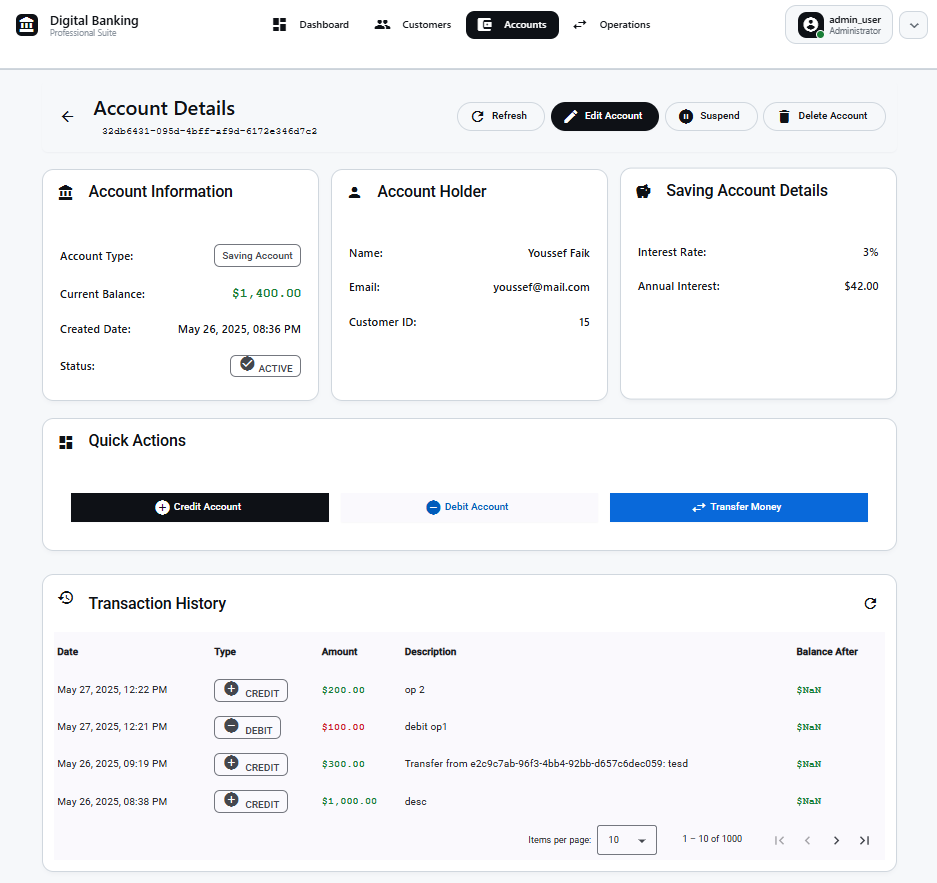
\includegraphics[width=0.9\textwidth]{screenshots/06_06_account_details_after_credit.png}
    \caption{\textbf{Compte après crédit} - Solde augmenté et nouvelle opération dans l'historique}
    \label{fig:account_details_after_credit}
\end{figure}

\subsection{Opérations de Virement}

\subsubsection{Formulaire de Virement}

Interface pour effectuer des virements entre comptes avec sélection des comptes source et destination.

\begin{figure}[H]
    \centering
    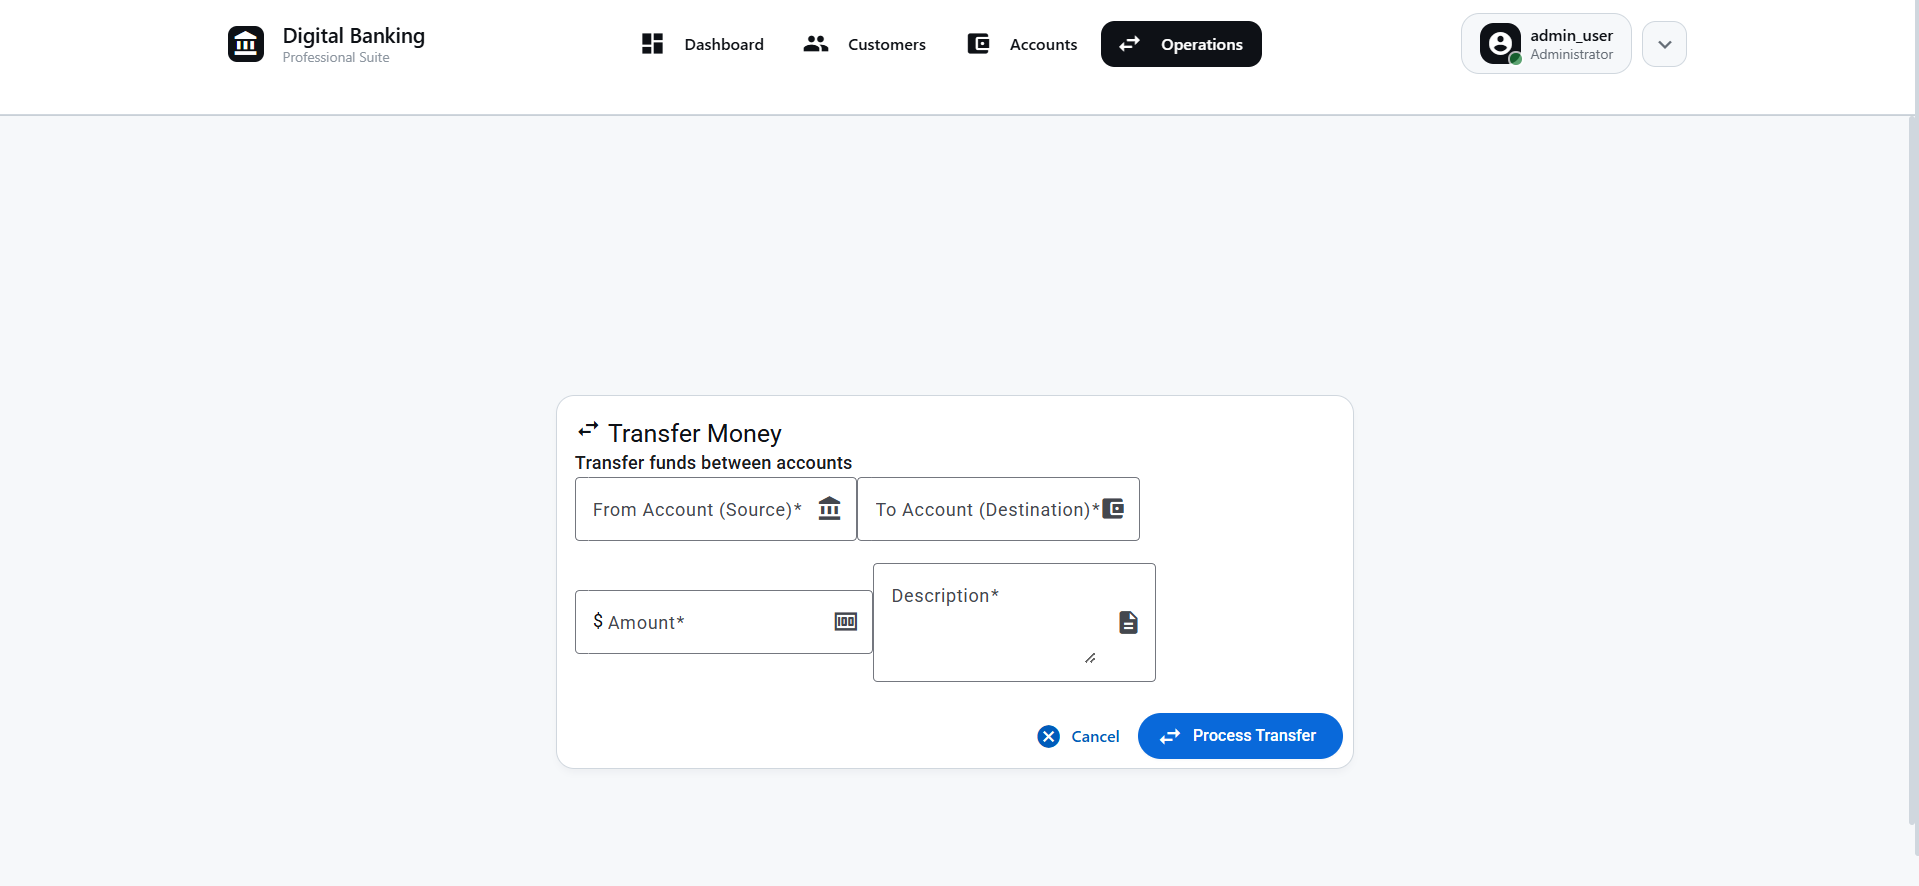
\includegraphics[width=0.75\textwidth]{screenshots/06_07_operation_transfer_form_empty.png}
    \caption{\textbf{Formulaire de virement} - Interface pour transfert entre comptes}
    \label{fig:operation_transfer_form_empty}
\end{figure}

\subsubsection{Exécution du Virement}

Exemple de virement de 300€ entre deux comptes avec description de l'opération.

\begin{figure}[H]
    \centering
    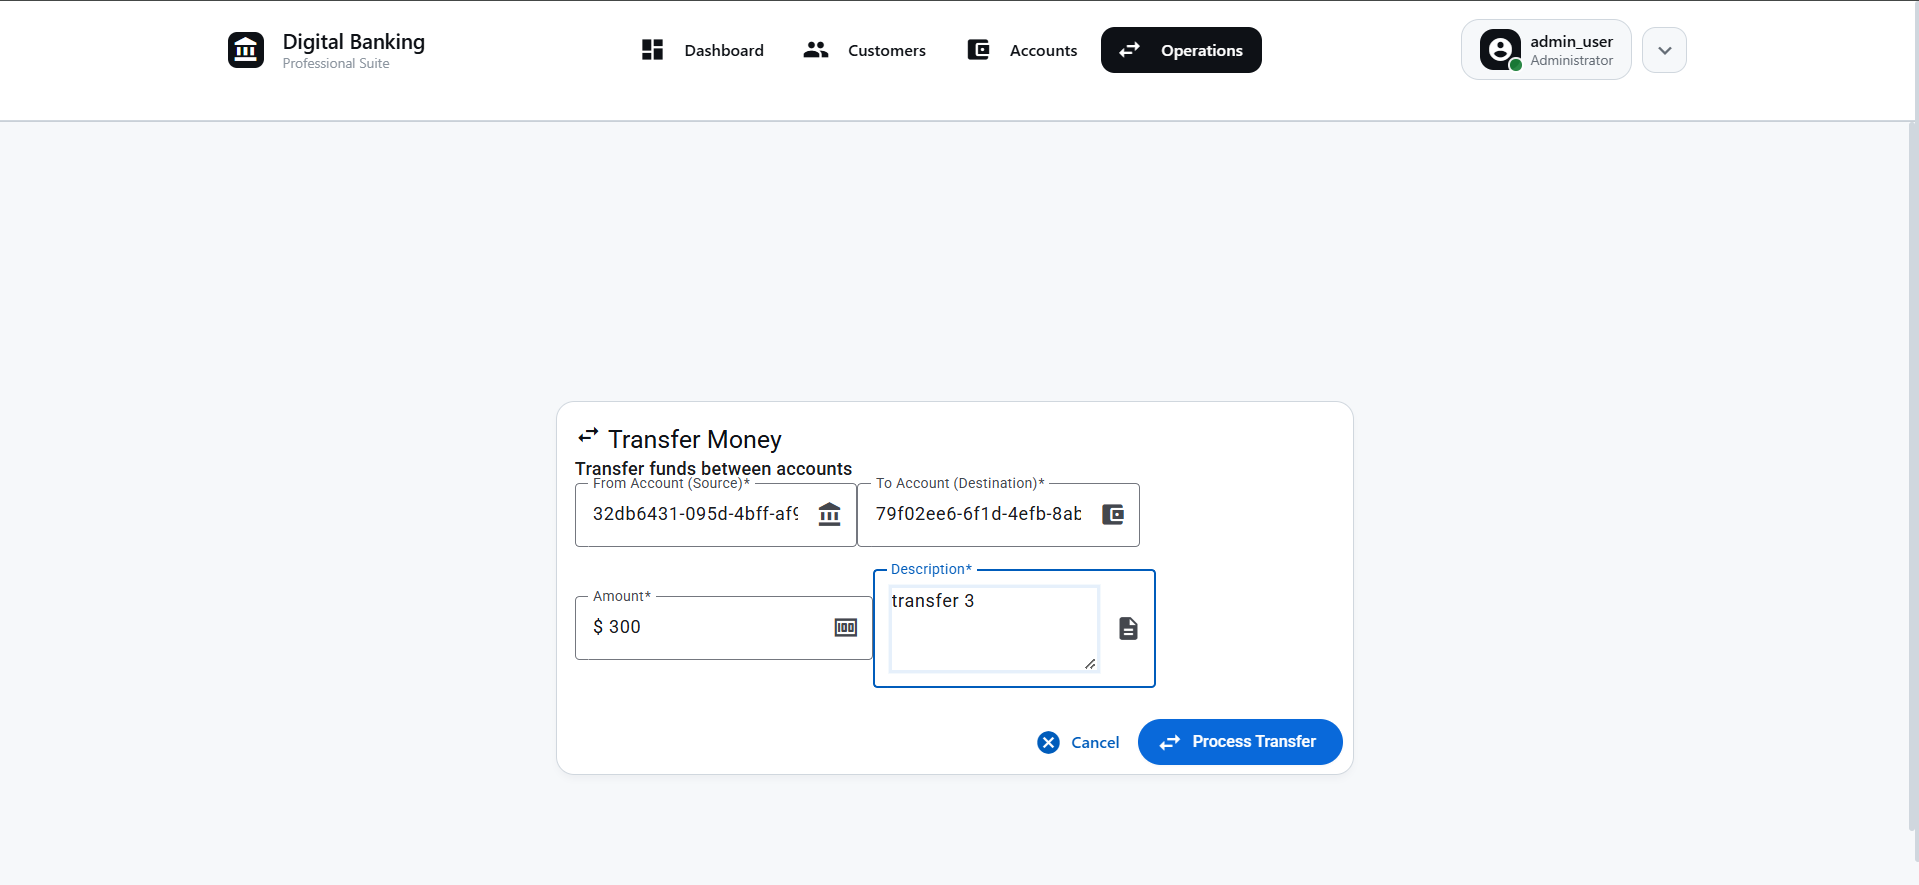
\includegraphics[width=0.75\textwidth]{screenshots/06_08_operation_transfer_form_filled.png}
    \caption{\textbf{Virement configuré} - Montant, comptes et description définis}
    \label{fig:operation_transfer_form_filled}
\end{figure}

\subsubsection{Résultat du Virement}

État du compte après virement avec solde ajusté et enregistrement de l'opération.

\begin{figure}[H]
    \centering
    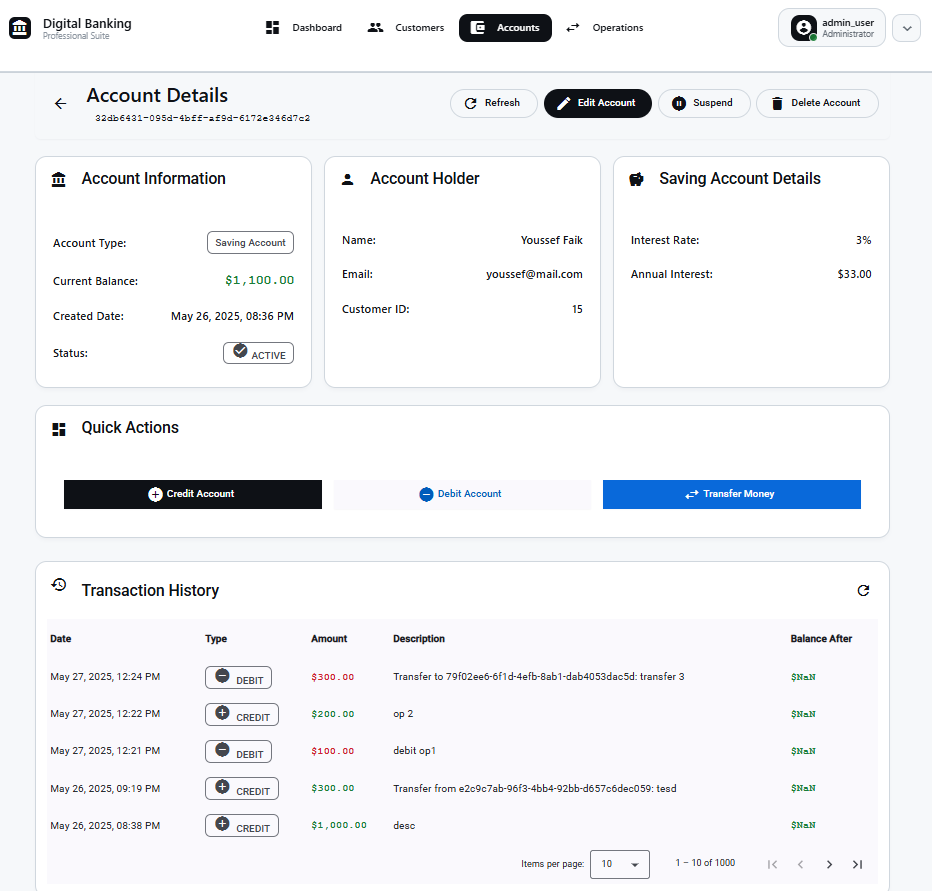
\includegraphics[width=0.9\textwidth]{screenshots/06_09_account_details_after_transfer.png}
    \caption{\textbf{Compte après virement} - Solde modifié et virement enregistré dans l'historique}
    \label{fig:account_details_after_transfer}
\end{figure}

\section{Conclusion}
\accentline

L'application \textbf{Digital Banking} présente un écosystème bancaire numérique complet et moderne, démontrant l'efficacité des technologies contemporaines pour créer une expérience utilisateur fluide et sécurisée.

\subsection{Points Forts de l'Application}

\begin{itemize}[leftmargin=20pt, itemsep=5pt]
    \item \textbf{Interface Moderne} : Design épuré et ergonomique favorisant l'expérience utilisateur
    \item \textbf{Sécurité Robuste} : Système d'authentification sécurisé avec gestion d'erreurs appropriée
    \item \textbf{Fonctionnalités Complètes} : Gestion intégrale des clients, comptes et opérations bancaires
    \item \textbf{Traçabilité} : Historique détaillé de toutes les opérations avec horodatage
    \item \textbf{Validation} : Contrôles en temps réel et validation des données saisies
\end{itemize}

\subsection{Technologies et Architecture}

Cette documentation technique illustre la capacité de l'application à répondre aux besoins opérationnels d'une institution bancaire moderne, avec un focus particulier sur :

\begin{itemize}[leftmargin=20pt, itemsep=5pt]
    \item L'architecture moderne Angular/Spring Boot
    \item La sécurité des transactions et des données
    \item L'ergonomie et l'intuitivité de l'interface
    \item La traçabilité complète des opérations
\end{itemize}

L'ensemble des fonctionnalités présentées démontre la maturité de la solution et sa capacité à supporter les besoins d'une plateforme bancaire digitale professionnelle.

\end{document}
